\chapter{Perancangan}
\label{chap:perancangan}

Pada bab ini akan dijelaskan mengenai perancangan aplikasi yang akan dibangun meliputi diagram kelas rinci beserta deskripsi dan fungsinya, dan perancangan antarmuka.

\section{Perancangan Sequence Diagram}

Pada \textit{sequence} diagram akan dibahas mengenai jalannya koneksi \textit{socket.io} dari awal koneksi mulai tersambung hingga koneksi terputus.

\subsection{Sequence Diagram Join Room}

\begin{figure}[H]
	\centering
	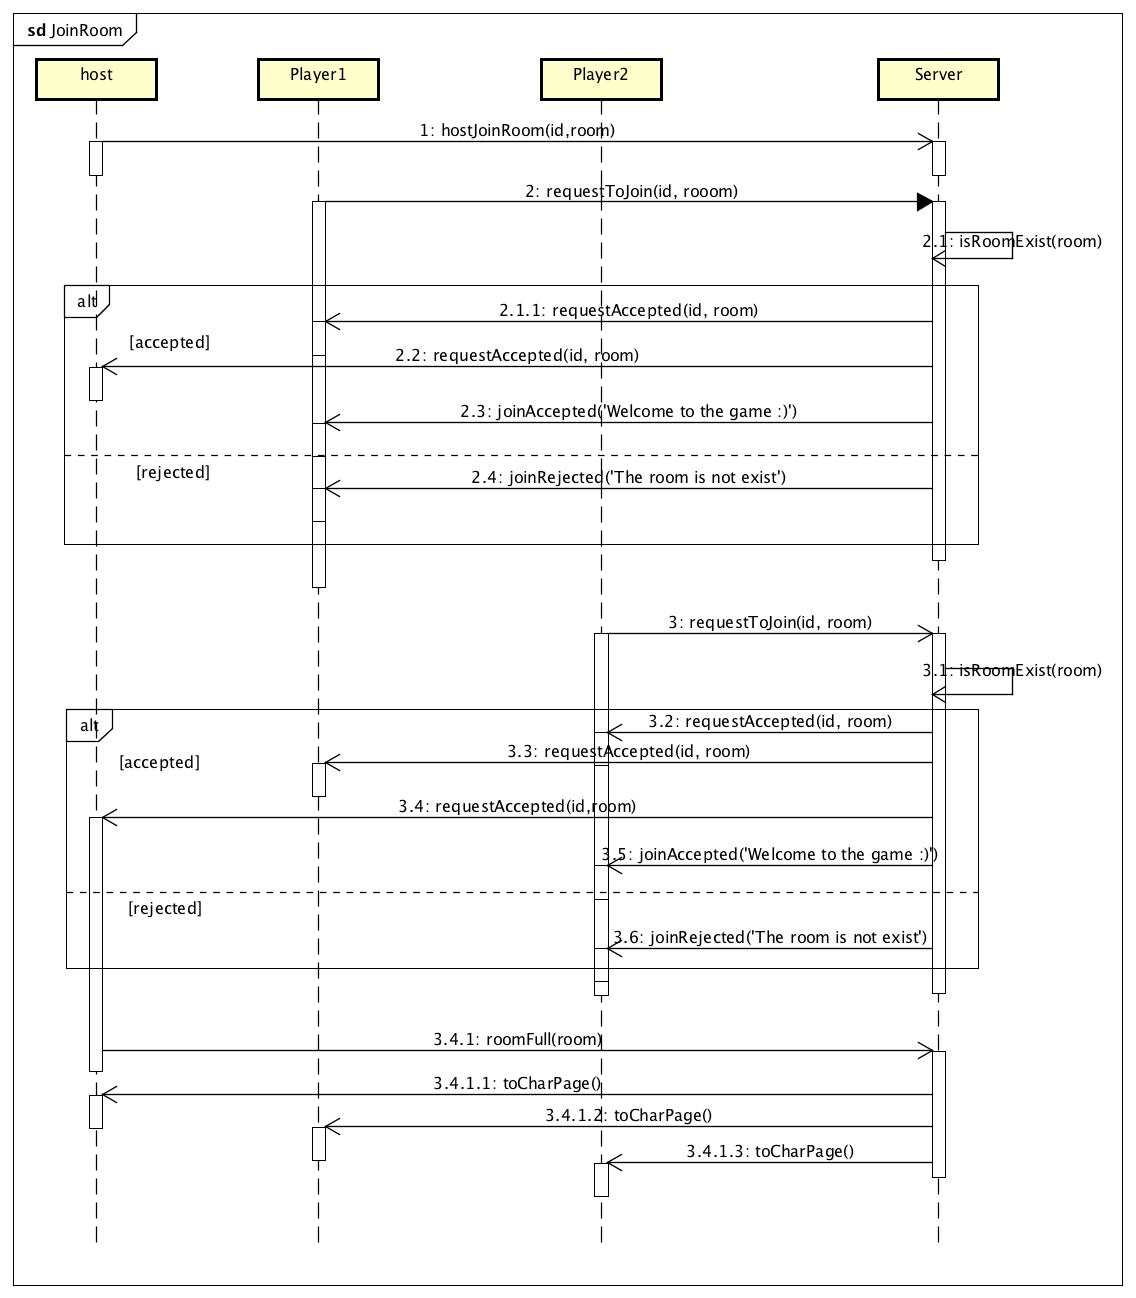
\includegraphics[scale=0.3]{Gambar/JoinRoom}
	\caption{Proses melakukan koneksi ke \textit{socket.io} dan bergabung kedalam \textit{room}.}
	\label{fig:1_JoinRoom}
\end{figure}

Pada awal permainan, \textit{client} pertama yang melakukan koneksi pada \textit{server} adalah \textit{desktop computer}, yang berperan sebagai \textit{host} dalam permainan.\textit{Host} akan menyediakan suatu kode yang berguna sebagai \textit{room} untuk kedua pemain yang akan bergabung dengan melakukan koneksi ke \textit{server}. \textit{Room} yang disediakan hanya akan menerima tiga \textit{client} saja, yaitu \textit{host}, \textit{player1}, dan \textit{player2}.

\textit{Host} akan mengirimkan \textit{event} yang menandakan akan bergabung kedalam room, \textit{event} tersebut adalah \textbf{hostJoinRoom(id, room)}. \textit{Event} ini memiliki data yang akan dikirimkan kepada \textit{server}, data-data tersebut dijelaskan sebagai berikut:
\begin{itemize}
	\item \textbf{id} identifikasi unik yang dimiliki masing-masing \textit{client} yang terkoneksi dengan \textit{socket.io}.
	\item \textbf{room} suatu \textit{string} yang menandakan ruangan dimana \textit{client} hanya akan melakukan komunikasi didalam ruangan tersebut.
\end{itemize}
Data-data tersebut akan dimasukan kedalam suatu \textit{array}, dimana \textit{array} tersebut akan menyimpan seluruh \textit{client} yang terkoneksi dengan \textit{socket.io}.

Setelah \textit{host} terkoneksi dengan \textit{socket.io}, maka \textit{room} milik \textit{host} sudah tersedia dan para pemain dapat bergabung kedalam \textit{room} tersebut. Untuk dapat mulai bermain, para pemain harus memasukan kode \textit{room} yang disediakan di halaman \textit{host}. Pemain akan mengirimkan \textit{event} \textbf{requestToJoin(id, room)} pada \textit{server}. Data yang dikirimkan oleh pemain sama dengan data yang dikirimkan oleh \textit{host}. 

Setelah \textit{event} tersebut diterima oleh \textit{server}, maka akan dilakukan pengecekan apakah pemain dapat bergabung atau tidak kedalam \textit{room}. Pengecekan tersebut dilakukan dengan menggunakan \textit{method} \textbf{isRoomExist(room)}. Beberapa pengecekan yang dilakukan \textit{method} ini akan dijelaskan sebagai berikut:
\begin{enumerate}
	\item Memeriksa apakah data \textit{room} didalam \textit{array} ada yang sesuai dengan parameter \textit{room}.
	\item Memeriksa apakah jumlah yang ada didalam \textit{room} yang dimaksud sudah lebih dari tiga atau belum.
\end{enumerate}

Apabila kedua hal diatas terpenuhi, maka pemain akan terkoneksi ke \textit{socket.io} dan bergabung ke dalam \textit{room}. \textit{Server} akan mengirimkan \textit{event} \textbf{requestAccepted(id, room)} kepada seluruh \textit{client} yang berada di \textit{room} tersebut. \textit{Event} tersebut berfungsi untuk mencatat \textit{client} telah berhasil bergabung kedalam room.\textit{Server} pun akan mengirimkan \textit{event} \textbf{joinAccepted('Welcome to the game :)')} kepada pemain yang berhasil bergabung kedalam \textit{room}. \textit{Event} tersebut berfungsi untuk memberikan \textit{feedback} kepada pemain bahwa pemain telah berhasil bergabung kedalam permainan.

Apabila kedua hal diatas tidak terpenuhi, maka pemain tidak dapat terkoneksi ke \textit{socket.io}. \textit{Server} akan mengirimkan \textit{event} \textbf{joinRejected('The room is not exist')} kepada pemain. \textit{Event} tersebut berfungsi sebagai \textit{feedback} kepada pemain yang tidak dapat bergabung. Pemain pertama yang berhasil bergabung akan berperan sebagai \textit{Player1}. Setelah satu pemain bergabung, maka \textit{server} akan menunggu untuk pemain kedua agar permainan dapat dimulai. Pemain kedua akan melakukan hal yang sama dengan pemain pertama untuk dapat bergabung kedalam room.

Setelah \textit{room} berisi tiga \textit{client}, maka \textit{host} akan mengirimkan \textit{event} \textbf{roomFull(room)} kepada \textit{server}. \textit{Event} tersebut menandakan bahwa \textit{room} sudah tidak dapat menerima \textit{client} yang akan bergabung. Setelah \textit{event} tersebut diterima oleh \textit{server}, maka \textit{event} \textbf{toCharPage()} akan dipancarkan oleh \textit{server} kepada seluruh koneksi yang ada didalam \textit{room} tersebut. \textit{Event} ini berfungsi untuk mengganti halaman saat ini ke halaman selanjutnya.

\subsection{Sequence Diagram Choose Character}

\begin{figure}[H]
	\centering
	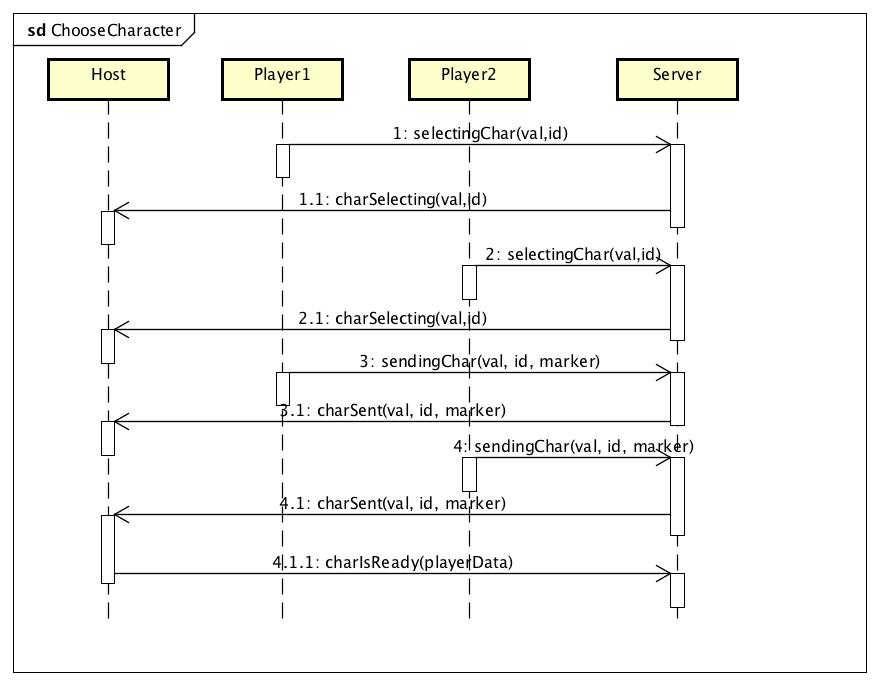
\includegraphics[scale=0.3]{Gambar/ChooseCharacter}
	\caption{Proses memilih karakter.}
	\label{fig:2_ChooseCharacter}
\end{figure}

Halaman ini merupakan halaman yang dituju oleh para pemain yang telah berhasil melakukan koneksi dan bergabung kedalam \textit{room}. Para pemain akan memilih karakter yang ada pada halaman \textit{smartphone browser}, dimana karakter yang dipilih akan muncul pada halaman \textit{desktop browser}. Pemain yang memilih karakter tertentu akan mengirimkan \textit{event} \textbf{selectingChar(val, id)} kepada \textit{server}. Data-data yang dikirimkan akan dijelaskan sebagai berikut:
\begin{itemize}
	\item \textbf{val} identifikasi unik yang dimiliki oleh masing-masing karakter.
	\item \textbf{id} identifikasi unik yang dimiliki masing-masing \textit{client} yang terkoneksi dengan \textit{socket.io}.
\end{itemize}
Setelah \textit{event} tersebut diterima oleh \textit{server}, maka server akan mengirimkan \textit{event} \textbf{charSelecting(val, id)} kepada \textit{host}. \textit{Event} tersebut berfungsi untuk menampilkan karakter yang dipilih oleh pemain dihalaman \textit{desktop}.

Apabila pemain akan menetapkan karakter yang telah ditampilkan dihalaman \textit{desktop}, maka \textit{pemain} akan mengirimkan \textit{event} \textbf{sendingChar(val,id,marker)} kepada \textit{server}. Data-data tersebut sama seperti yang dikirimkan oleh \textit{event} sebelumnya, hanya saja ada tambahan data \textbf{marker} pada parameter. Data tersebut berfungsi sebagai penanda bahwa sudah ada satu pemain yang telah menetapkan karakter yang akan dimainkan. Setelah \textit{server} menerima \textit{event} tersebut, maka \textit{server} akan meneruskan data-data tersebut pada \textit{host} dengan mengirimkan \textit{event} \textbf{charSent(val,id,marker)}.

Pemain kedua pun akan melakukan hal yang sama untuk memilih dan menetapkan karakter yang akan dimainkan. Apabila kedua pemain telah menetapkan karakter yang akan dimainkan, \textit{host} akan memancarkan \textit{event} \textbf{charIsReady(playerData)}.Data yang dikirimkan merupakan suatu \textit{object array} yang berisi data para pemain dan data karakter yang telah dipilih.\textit{Event} tersebut berfungsi untuk memberi informasi kepada \textit{server} untuk pindah kehalaman selanjutnya.

\subsection{Sequence Diagaram Game Begin}

\begin{figure}[H]
	\centering
	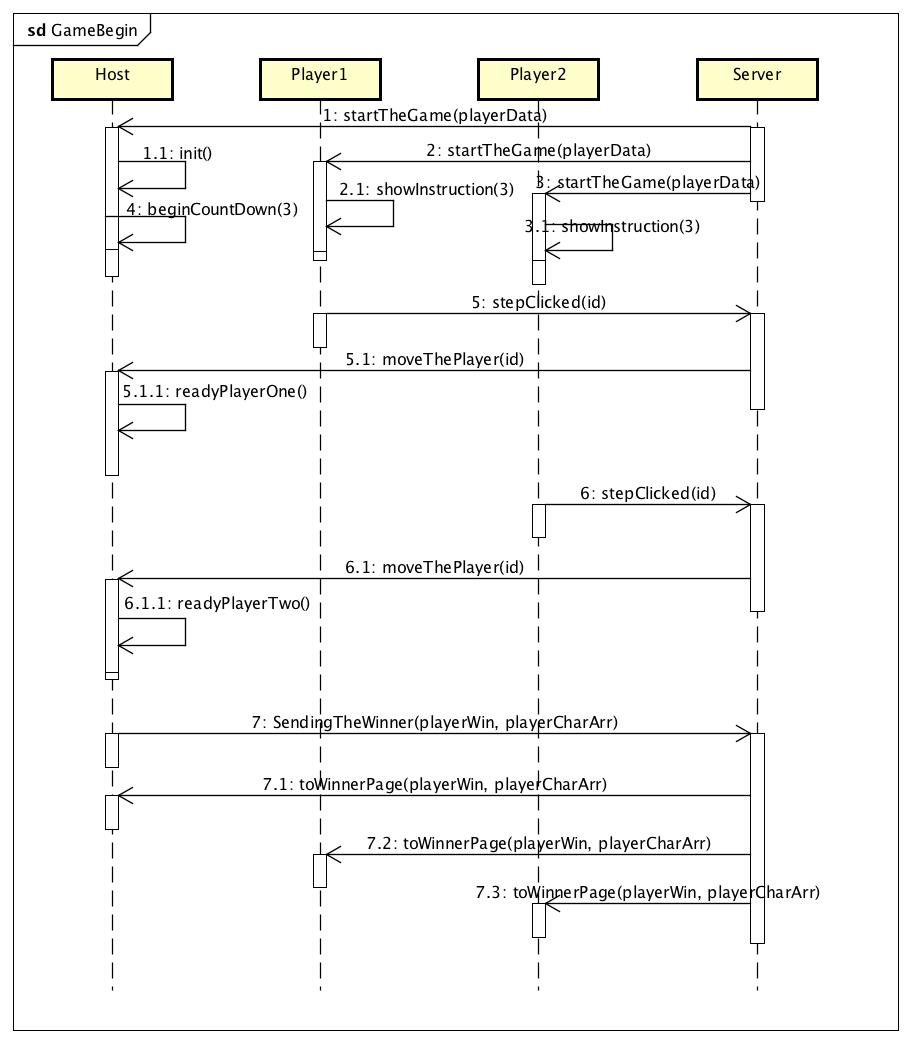
\includegraphics[scale=0.3]{Gambar/GameBegin}
	\caption{Proses memulai permainan.}
	\label{fig:3_GameBegin}
\end{figure}

Pada tahap ini, \textit{server} akan memancarkan \textit{event} \textbf{startTheGame(playerData)}. Data yang dikirimkan merupakan data yang didapatkan dari \textit{event} sebelumnya. \textit{Event} tersebut akan diterima oleh seluruh \textit{client} yang berada didalam \textit{room} tertentu, yang kemudian akan memulai permainannya. \textit{Host} akan mengeksekusi \textit{method} \textbf{init()} dan \textbf{beginCountDown(3)} untuk memulai permainan. \textit{Method} \textbf{init()} berfungsi untuk mulai menggambar lintasan lari di halaman saat ini yang akan menjadi tempat para karakter dimainkan. \textit{Method} \textbf{beginCountDown(3)} berfungsi untuk melakukan hitungan mundur selama tiga detik. 

Para pemain yang menerima \textit{event} \textbf{startTheGame(playerData)} akan mengeksekusi \textit{method} \textbf{showInstruction(3)}. \textit{Method} tersebut berfungsi untuk menampilkan instruksi untuk memainkan permainan selama tiga detik. Apabila hitungan mundur telah selesai, maka permainan akan dimulai.

Permainan dilakukan dengan cara menekan tombol-tombol yang ada pada halaman \textit{smartphone}. Apabila pemain menekan tombol, maka \textit{event} \textbf{stepClicked(id)} akan dipancarkan. \textit{Server} akan menerima \textit{event} tersebut, yang kemudian akan meneruskannya dengan memancarkan \textit{event} \textbf{moveThePlayer(id)} kepada \textit{host}. Setelah \textit{event} tersebut diterima oleh \textit{host}, maka \textit{host} akan menjalankan \textit{method} tertentu. Apabila \textit{Player1} yang menekan tombol, maka \textit{method} \textbf{readyPlayerOne()} akan dieksekusi oleh \textit{host}. Apabila \textit{Player2}, maka \textbf{readyPlayerTwo()} akan dieksekusi. Kedua \textit{Method} tersebut berfungsi untuk memindahkan posisi karakter milik pemain dari posisi semula hingga posisi tertentu. Permainan akan berakhir apabila ada karakter yang menyentuh garis akhir pertama kali.

Apabila ada pemain yang berhasil menyentuh garis akhir, maka \textit{host} akan memancarkan \textit{event} \textbf{sendingTheWinner(playerWin, playerCharArr)}. Data-data yang dikirimkan akan dijelaskan sebagai berikut:
\begin{itemize}
	\item \textbf{playerWin} angka \textit{integer} yang menandakan pemain nomor berapa yang memenangkan permainan.
	\item \textbf{playerCharArr} \textit{array} yang menyimpan karakter dari masing-masing pemain.
\end{itemize}
\textit{Server} akan menangkap \textit{event} tersebut dan meneruskannya dengan memancarkan \textit{event} \textbf{toWinnerPage(playerWin, playerCharArr)} ke setiap \textit{client} pada \textit{room} tertentu. \textit{Event} tersebut berfungsi untuk berpindah ke halaman selanjutnya.

\subsection{Sequence Diagram Winning Page}
\begin{figure}[H]
	\centering
	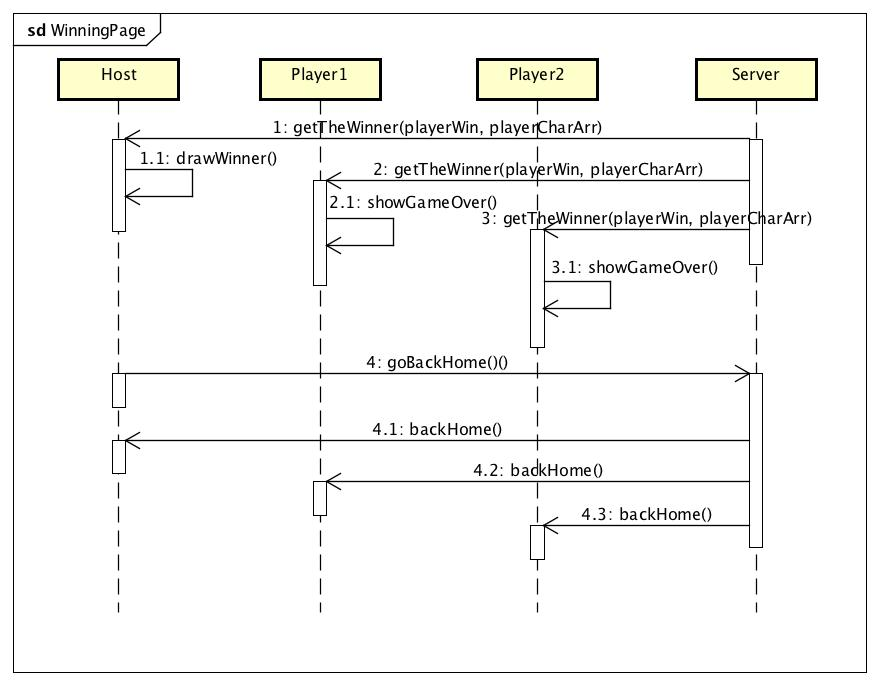
\includegraphics[scale=0.3]{Gambar/WinningPage}
	\caption{Menampilkan para pemain yang telah selesai bermain.}
	\label{fig:4_WinningPage}
\end{figure}

Pada tahap ini, \textit{server} akan memancarkan \textit{event} \textbf{getTheWinner(playerWin, playerCharArr)} dengan data-data yang diterima dari \textit{event} sebelumnya. \textit{Host} akan menerima \textit{event} tersebut dan akan mengeksekusi \textit{method} \textbf{drawWinner()}. \textit{Method} tersebut berfungsi untuk menampilkan karakter milik para pemenang yang telah selesai bermain. Para pemain akan menerima \textit{event} yang dipancarkan oleh \textit{server} dan mengeksekusi \textit{method} \textbf{showGameOver()}. \textit{Method} ini akan menampilkan teks yang menunjukan bahwa permainan telah selesai.

Apabila pemain menekan tombol \textit{back} yang ada pada halaman \textit{browser}, maka \textit{host} akan memancarkan \textit{event} \textbf{goBackHome()}. \textit{Event} tersebut akan diterima oleh \textit{server} dan akan diteruskan dengan memancarkan \textit{event} \textbf{backHome()}. Selurh \textit{client} didalam \textit{room} yang menerima \textit{event} tersebut akan kembali kehalaman semula dan koneksi pun akan terputus.


\section{Perancangan Antarmuka}
\label{sec:antarmuka}

Antarmuka yang dirancang terbagi menjadi dua bagian, yaitu antarmuka pada \textit{browser} yang ada di \textit{PC} dan \textit{smartphone}.

\begin{enumerate}
	\item Antarmuka halaman \textit{home}
	
	\textbf{PC}
	
	Halaman ini merupakan halaman utama yang pertama kali dituju oleh pengguna yang menggunakan \textit{PC}. Komponen halaman ini terdiri dari dua buah gambar jari yang melambangkan permainan, teks yang menunjukan nama permainan yaitu \textit{finger for life}, dan tombol \textit{start} yang digunakan untuk memulai permainan. Rancangan antarmuka halaman \textit{home} dapat dilihat pada Gambar \ref{fig:web1_home}

\begin{figure}[H]
	\centering
	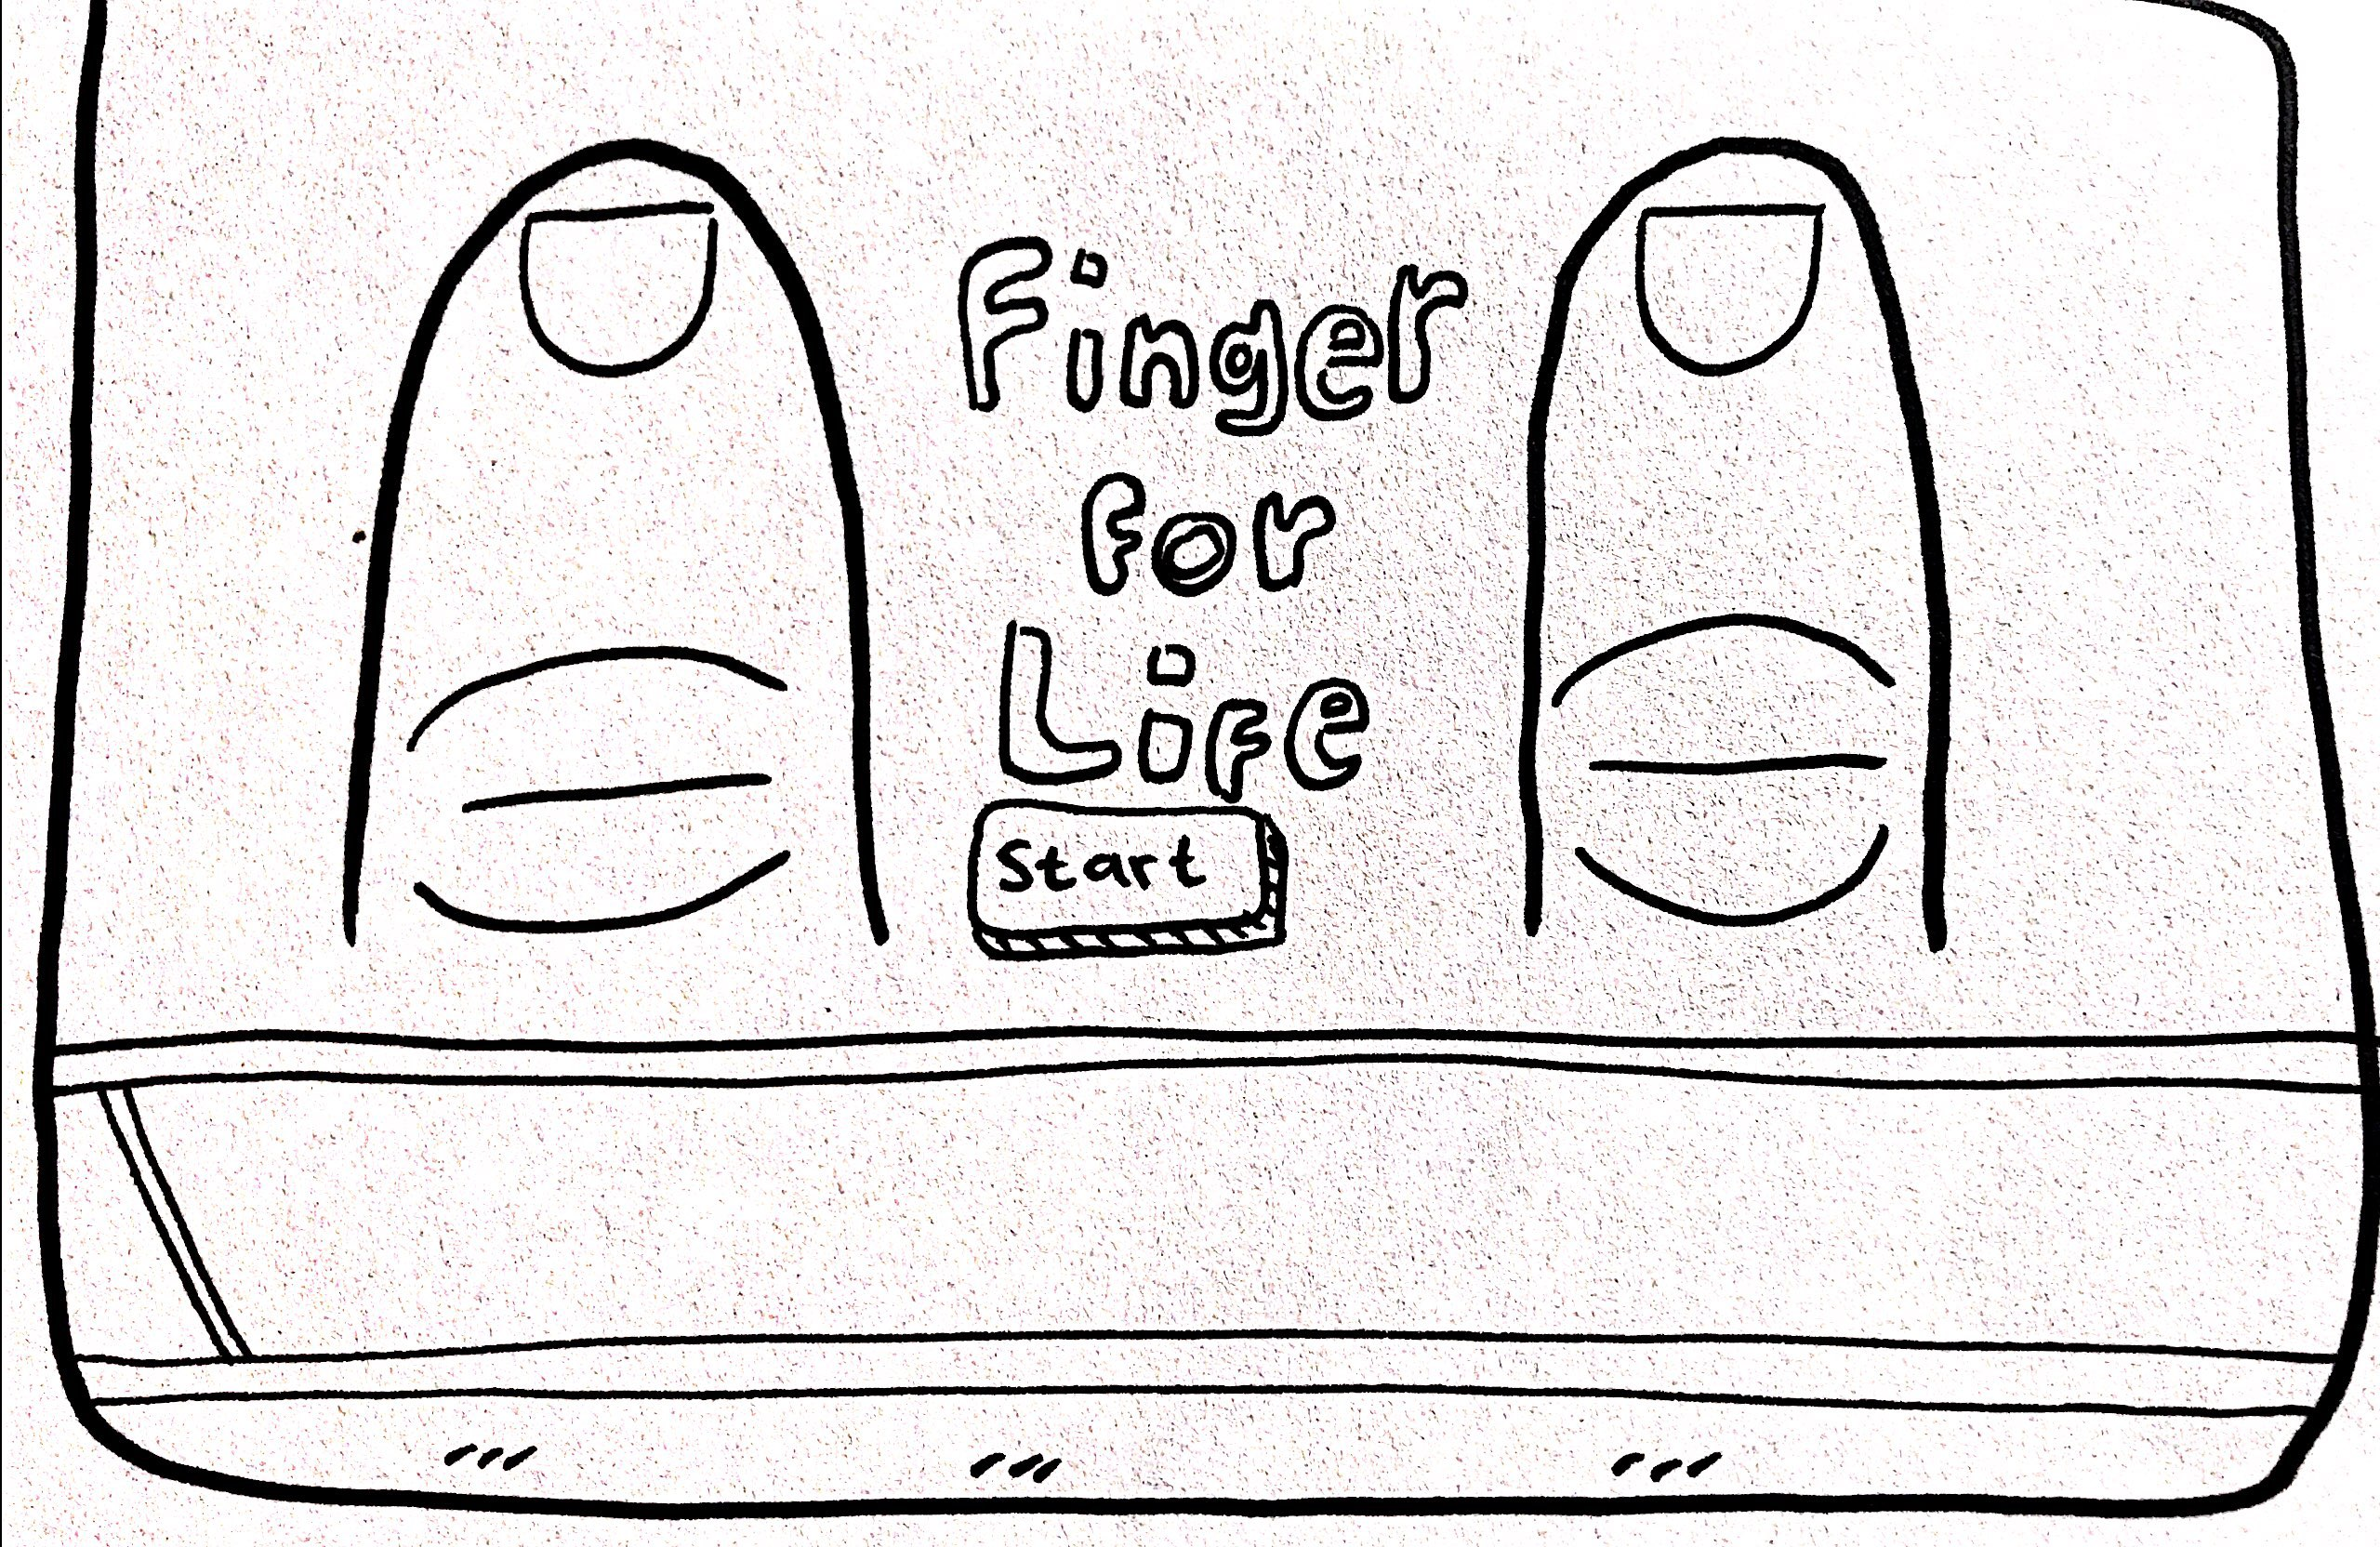
\includegraphics[scale=0.1]{Gambar/web1_home}
	\caption{Halaman pada \textit{PC} yang menunjukan berbagai permainan yang dapat dipilih.}
	\label{fig:web1_home}
\end{figure}

	\textbf{Smartphone}
	
	Halaman ini merupakan halaman utama yang pertama kali dituju oleh pengguna yang menggunakan \textit{smartphone}. Komponen halaman ini terdiri dari teks yang menunjukan nama permainan yaitu \textit{finger for life}, dan tombol \textit{join} yang digunakan untuk memulai permainan. Rancangan antarmuka halaman \textit{home} dapat dilihat pada Gambar \ref{fig:mob1_home}.
	
\begin{figure}[H]
	\centering
	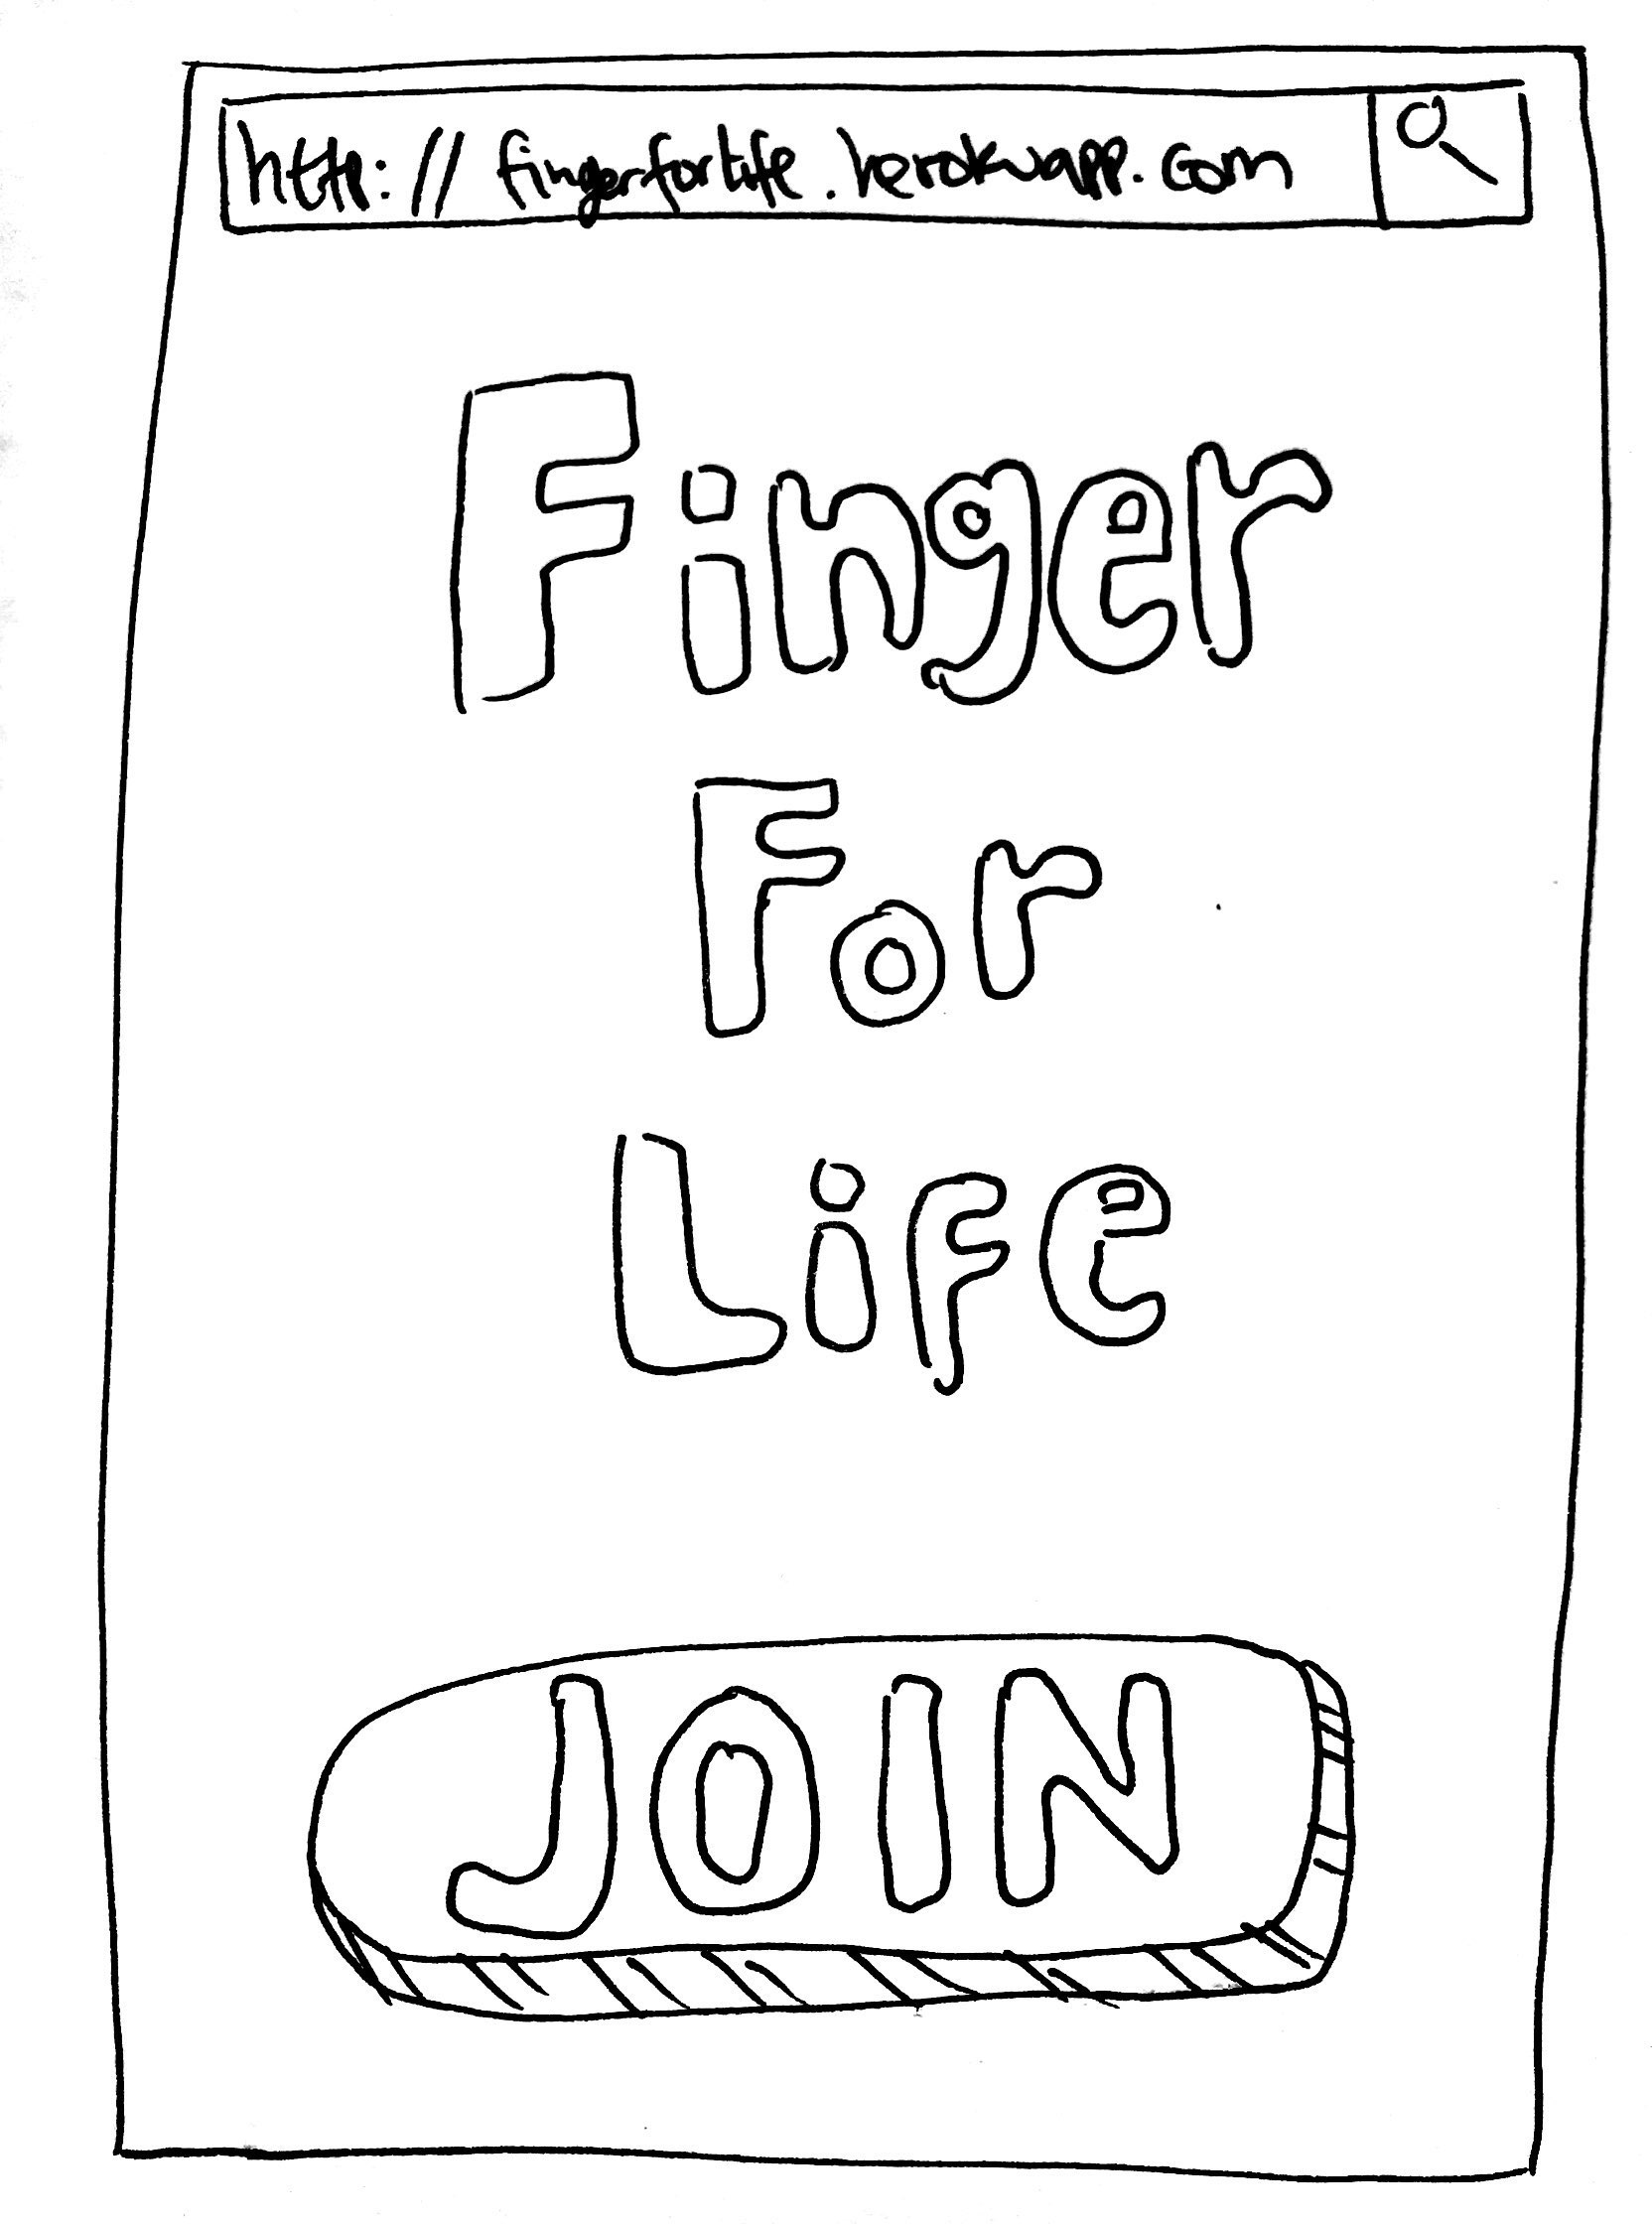
\includegraphics[scale=0.1]{Gambar/mob1_home}
	\caption{Halaman pada \textit{PC} yang menunjukan berbagai permainan yang dapat dipilih.}
	\label{fig:mob1_home}
\end{figure}

	\item Antarmuka halaman \textit{sync}
	
	\textbf{PC}
	
	Halaman ini menampilkan suatu perintah yang dapat dilakukan oleh pengguna apabila akan bergabung dalam permainan. Halaman ini pun menyediakan suatu kode untuk para pemain dimana kode tersebut akan berfungsi sebagai suatu \textit{room} bagi para pemain. Pada halaman ini akan dilakukan proses sinkronisasi untuk para pengguna, apakah berhasil bergabung dalam permainan atau tidak. Apabila berhasil, maka akan muncul suatu teks yang menunjukan suatu pemain telah berhasil bergabung. Apabila tidak, maka tidak akan menampilkan apapun dan halaman tidak akan menuju ke halaman selanjutnya sebelum ada dua pemain yang berhasil bergabung. Rancangan antarmuka halaman \textit{sync} pada \textit{PC} dapat dilihat pada Gambar \ref{fig:web2_sync}.
	
\begin{figure}[H]
	\centering
	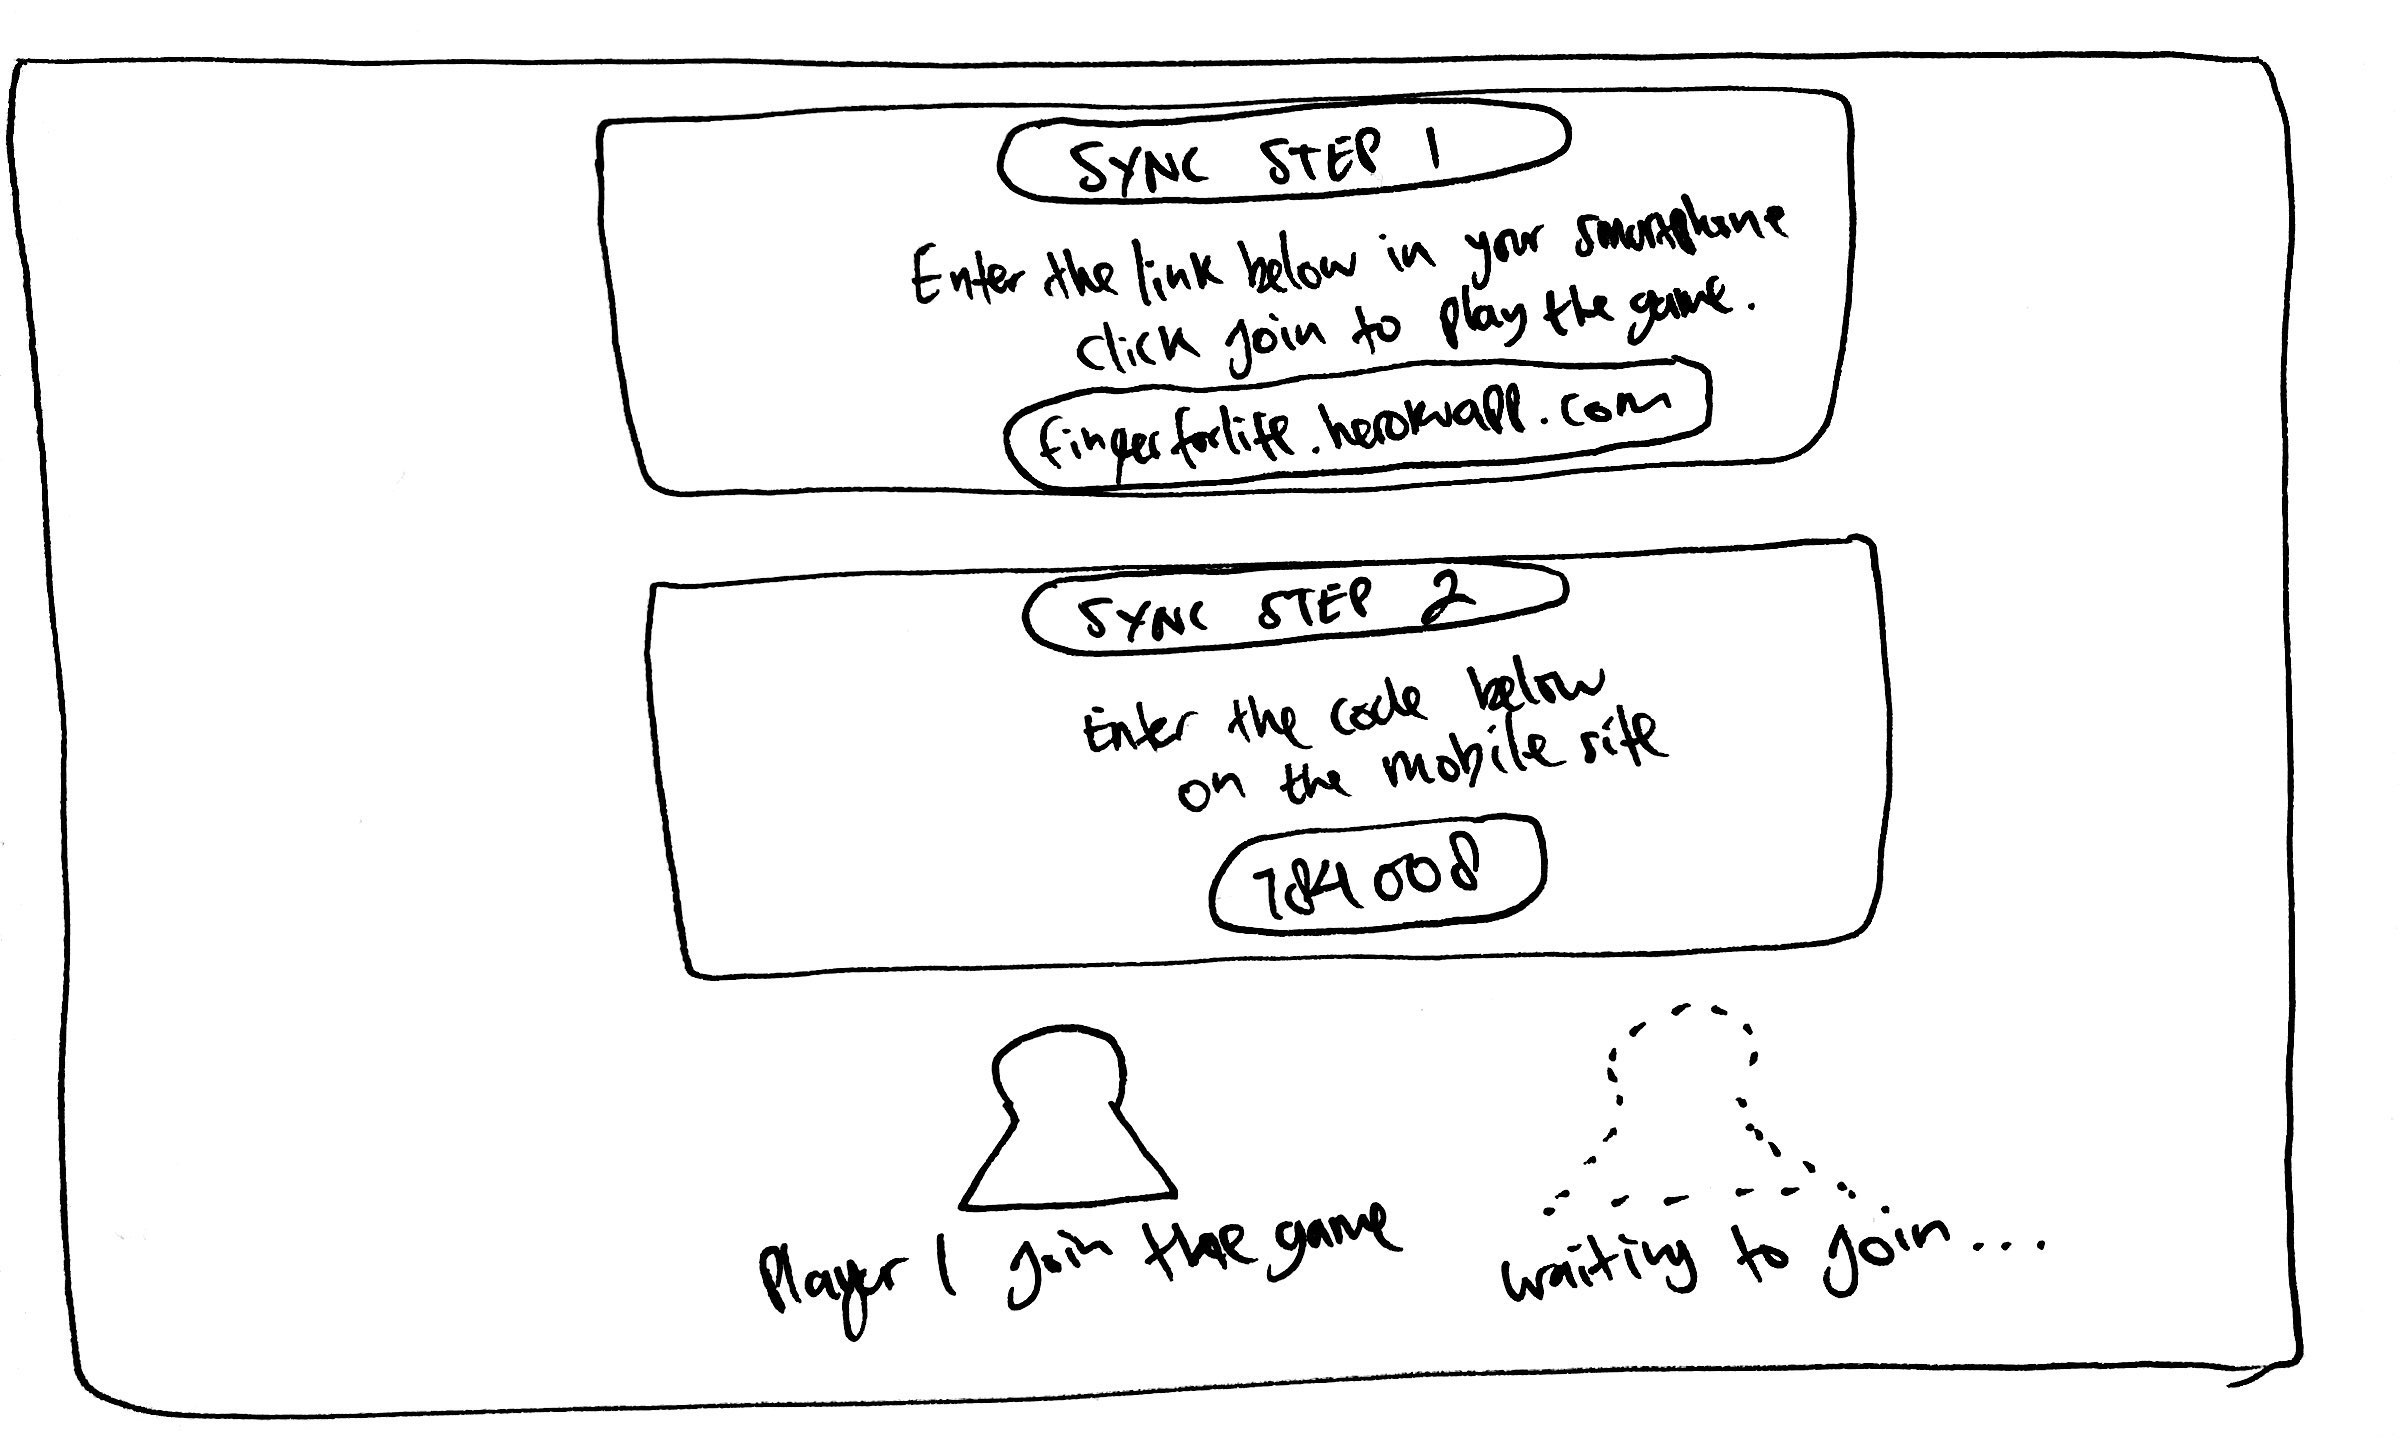
\includegraphics[scale=0.1]{Gambar/web2_sync}
	\caption{Halaman pada \textit{PC} yang menunjukan berbagai permainan yang dapat dipilih.}
	\label{fig:web2_sync}
\end{figure}

	\textbf{Smartphone}
	
	Halaman ini berfungsi untuk melakukan \textit{request} untuk bergabung dalam permainan. Komponen halaman ini terdiri dari kolom kode, dan tombol \textit{send}. Rancangan antarmuka halaman \textit{sync} pada \textit{smartphone} dapat dilihat pada Gambar \ref{fig:mob2_sync1}.
	
\begin{figure}[H]
	\centering
	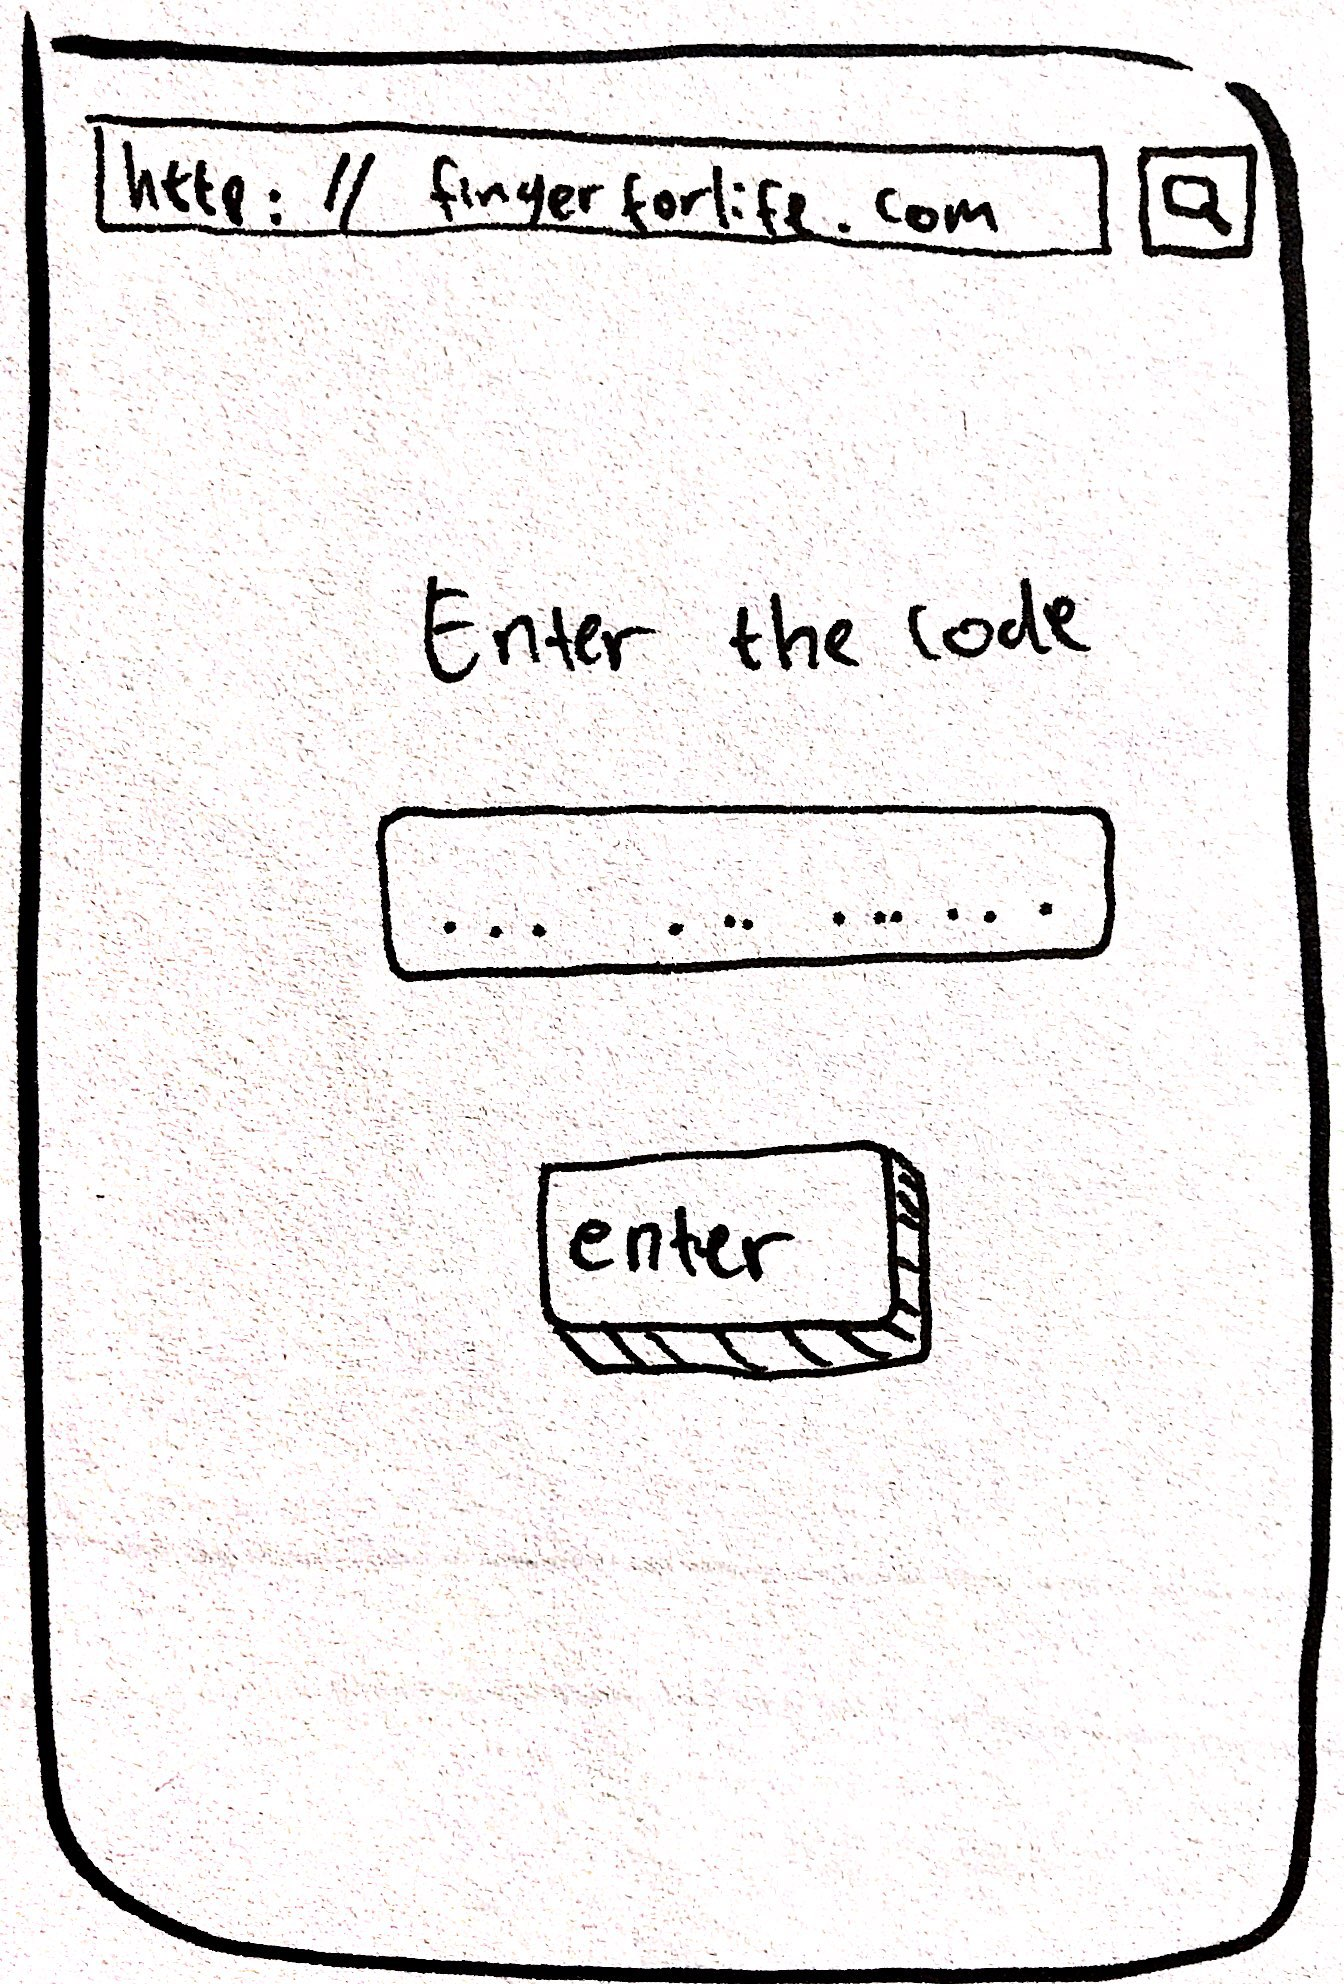
\includegraphics[scale=0.1]{Gambar/mob2_sync1}
	\caption{Halaman pada \textit{PC} yang menunjukan berbagai permainan yang dapat dipilih.}
	\label{fig:mob2_sync1}
\end{figure}

\item Antarmuka halaman \textit{character}

	\textbf{PC}
	
	Halaman ini akan menampilkan karakter yang telah dipilih oleh pemain. Apabila karakter belum memilih karakter yang akan dimainkan, maka halaman ini belum menampilkan apapun. Rancangan antarmuka halaman \textit{character} pada \textit{PC} dapat dilihat pada Gambar \ref{fig:web3_char}.
	
\begin{figure}[H]
	\centering
	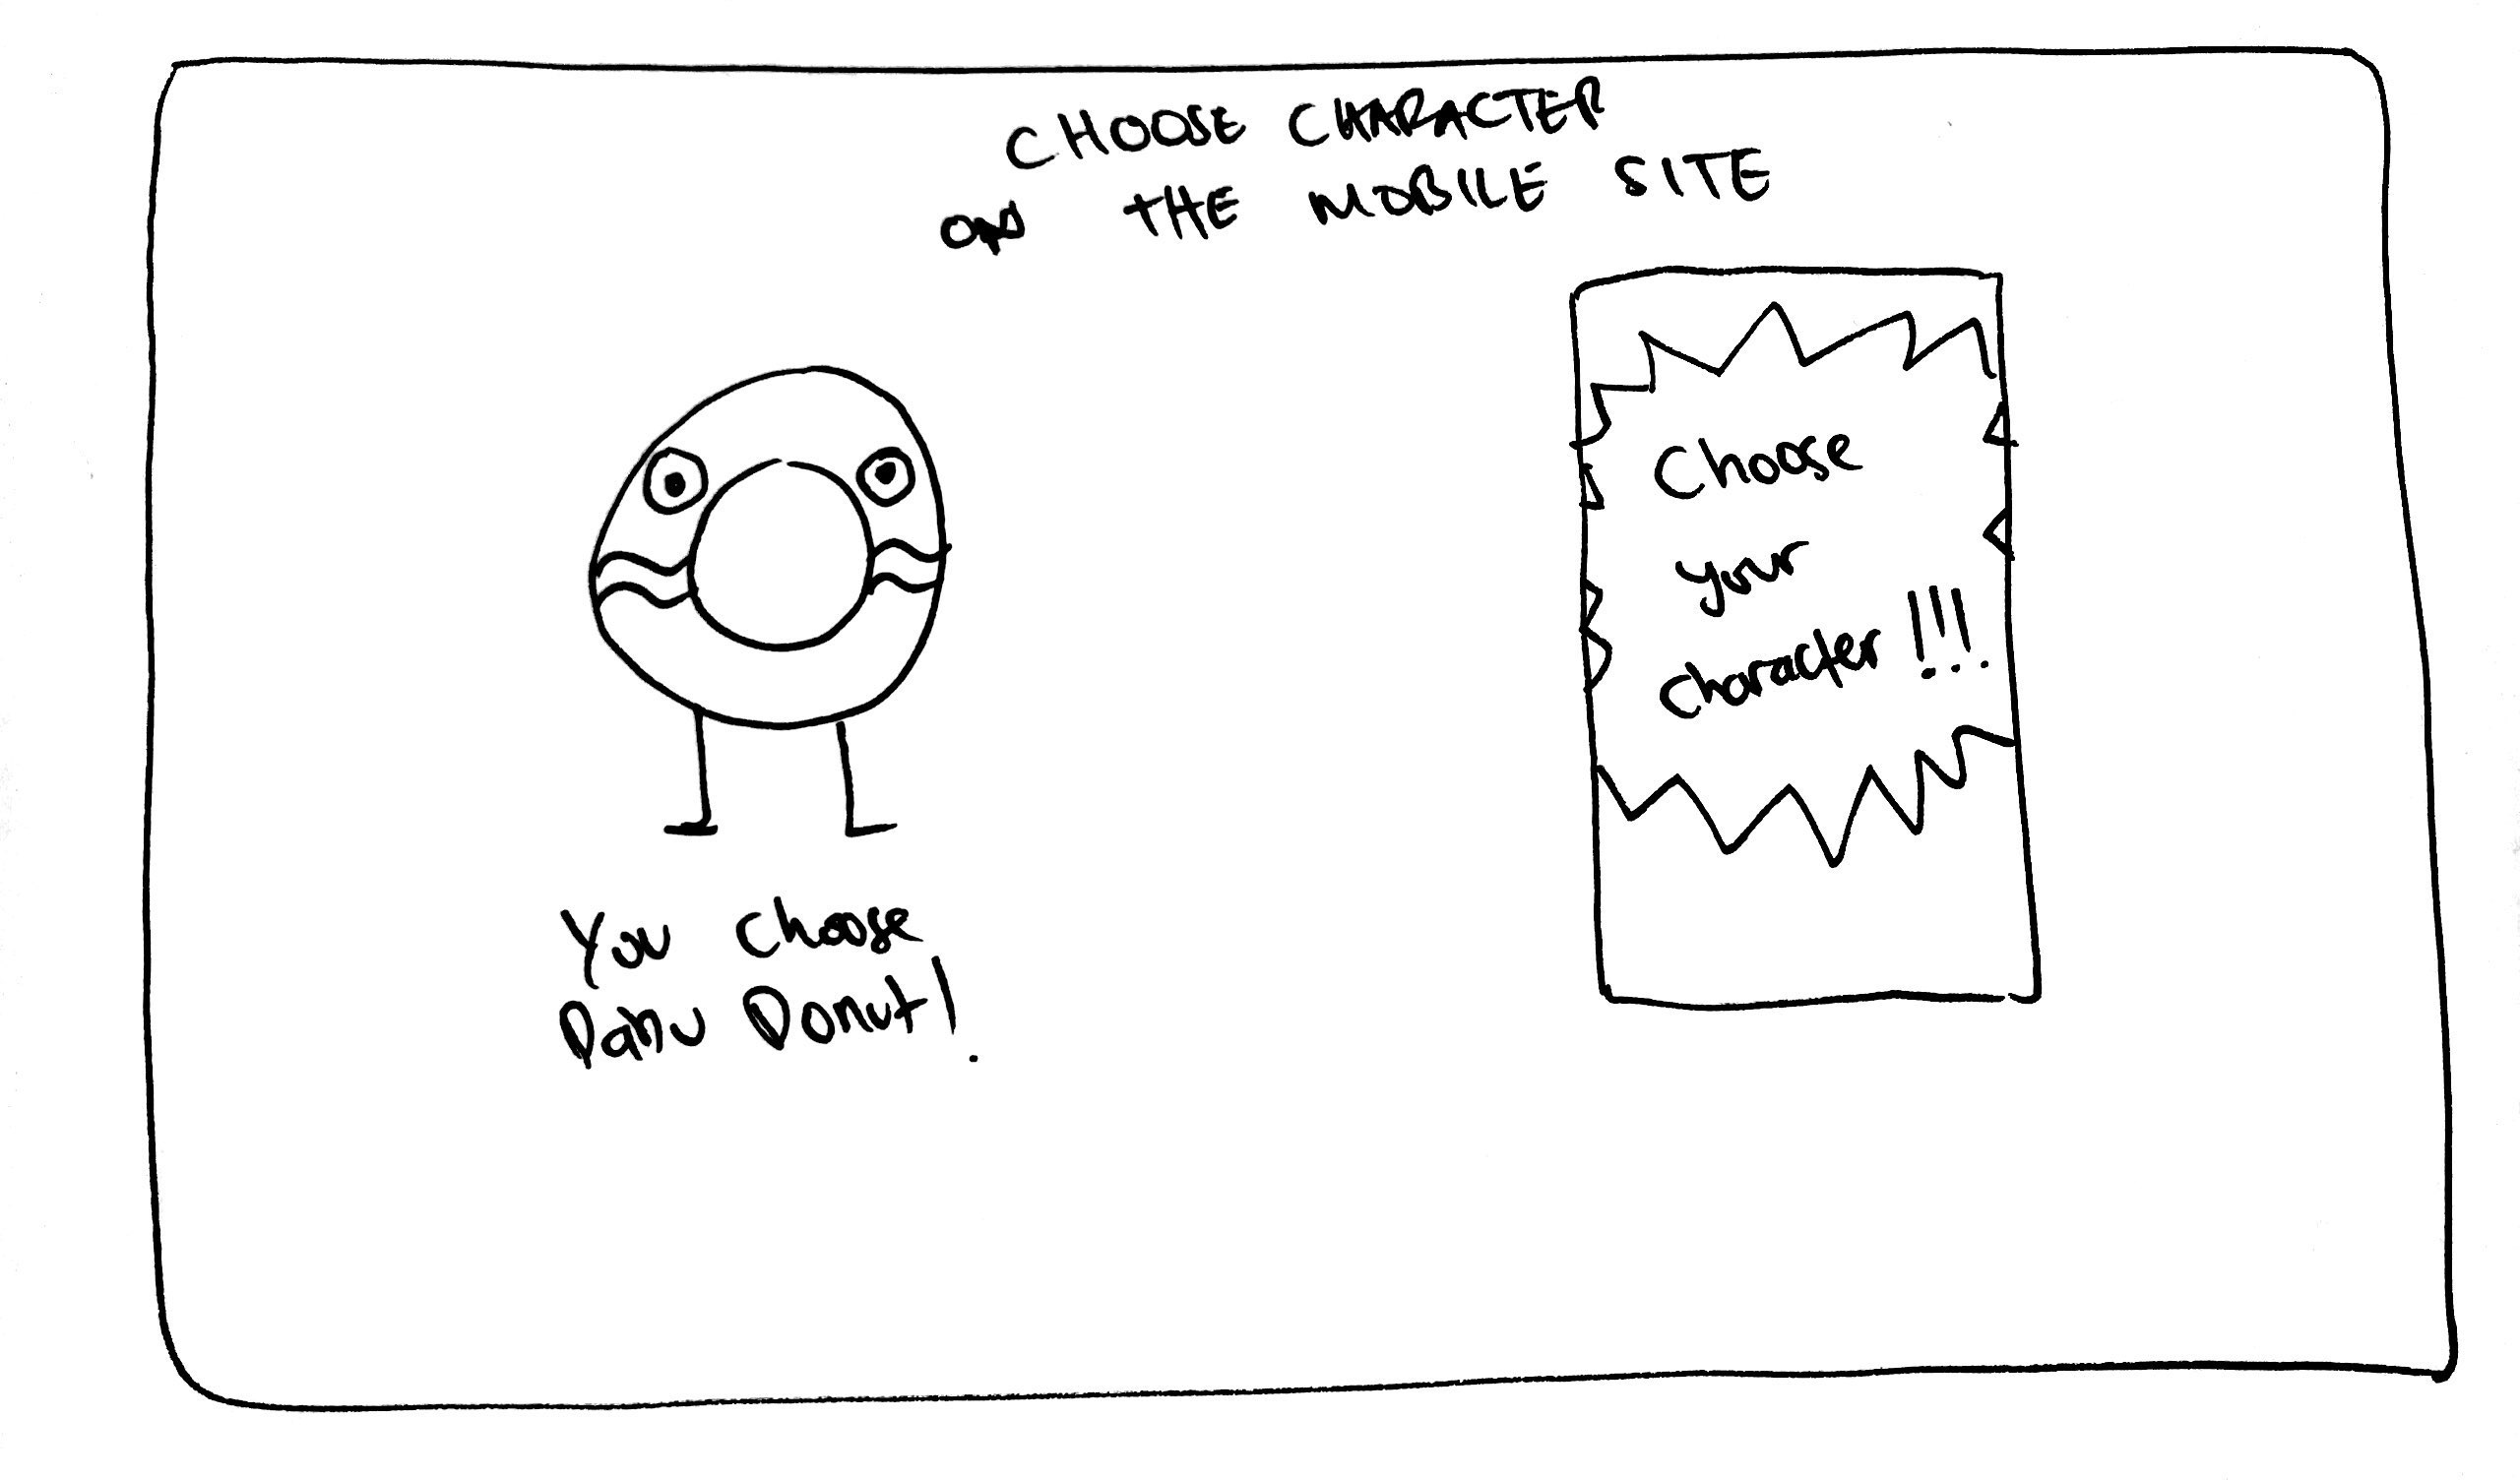
\includegraphics[scale=0.1]{Gambar/web3_char}
	\caption{Halaman pada \textit{PC} yang menunjukan berbagai permainan yang dapat dipilih.}
	\label{fig:web3_char}
\end{figure}


	\textbf{Smartphone}
	
	Halaman ini akan menampilkan daftar karakter yang dapat dimainkan oleh pemain. Komponen halaman ini terdiri dari daftar karakter, dan tombol \textit{choose}. Rancangan antarmuka halaman \textit{character} pada \textit{smartphone} dapat dilihat pada Gambar \ref{fig:mob3_char1}.
	
\begin{figure}[H]
	\centering
	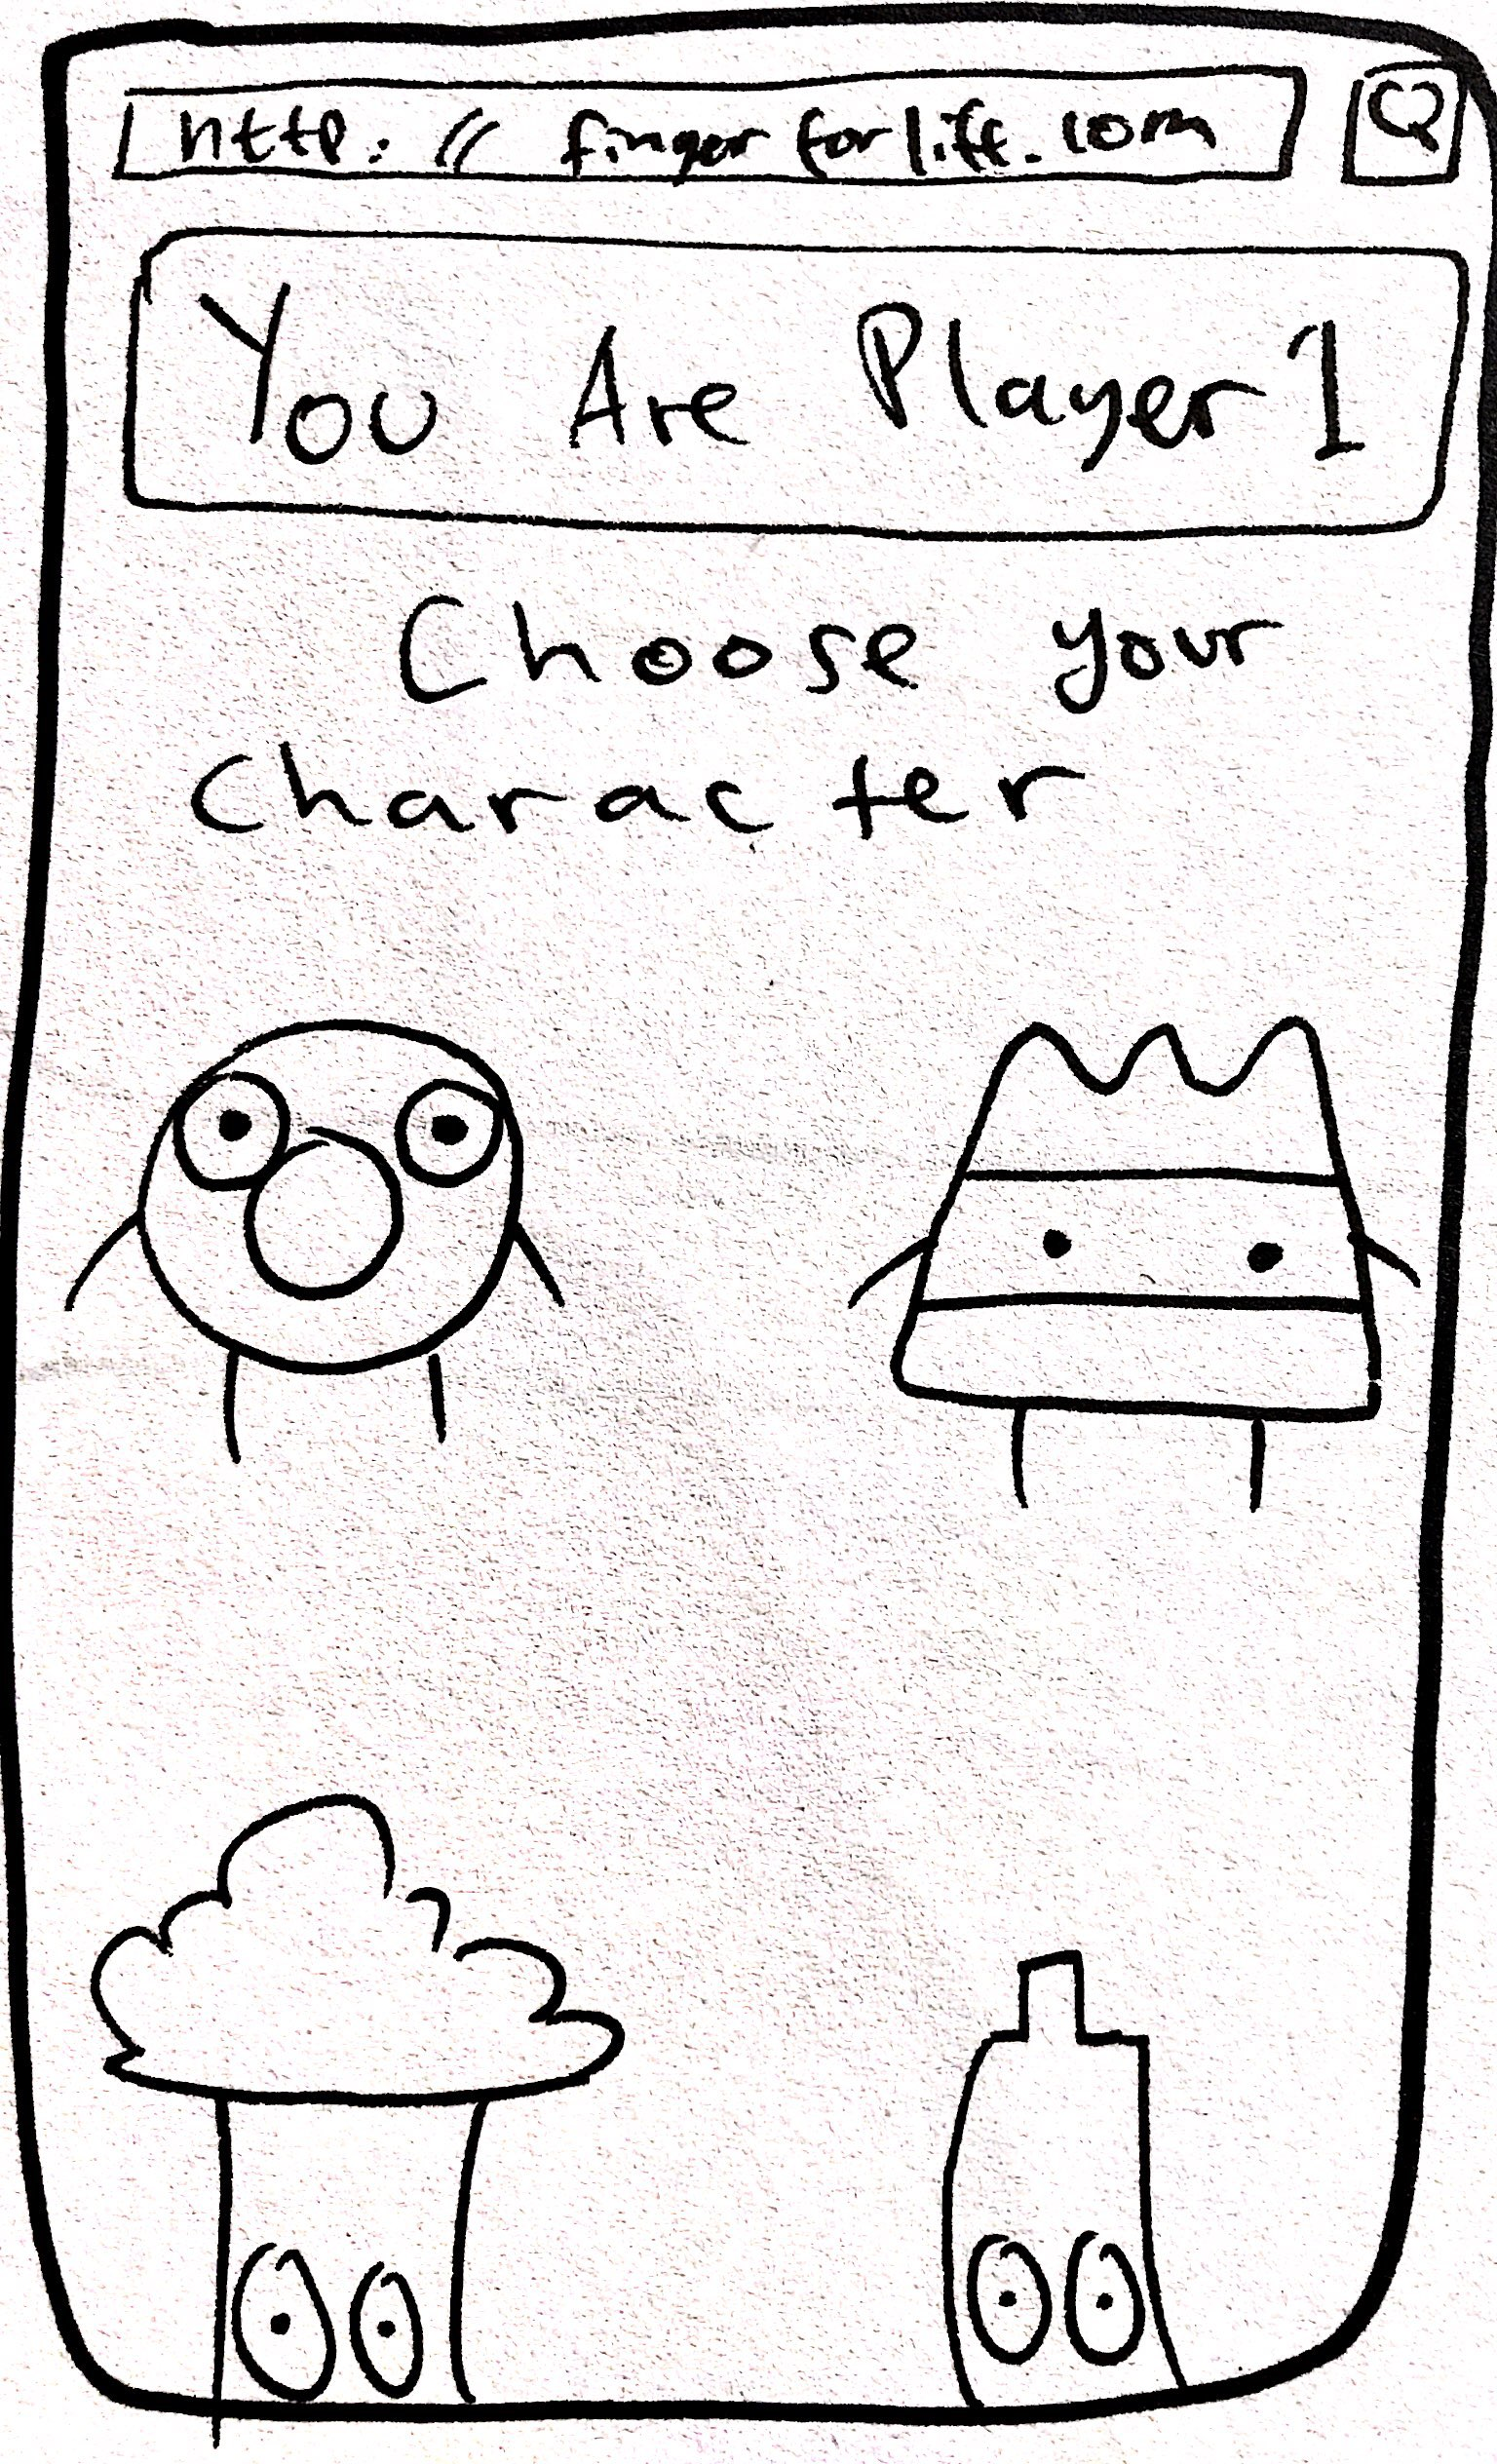
\includegraphics[scale=0.1]{Gambar/mob3_char1}
	\caption{Halaman pada \textit{PC} yang menunjukan berbagai permainan yang dapat dipilih.}
	\label{fig:mob3_char1}
\end{figure}

\item Antarmuka halaman \textit{gameplay}

	\textbf{PC}
	
	Halaman ini menampilkan arena permainan untuk para pemain. Komponen halaman ini terdiri dari suatu gambar lintasan lari, dan karakter yang telah dipilih pada halaman sebelumnya. Rancangan antarmuka halaman \textit{gameplay} pada \textit{PC} dapat dilihat pada Gambar \ref{fig:web5_gameplay2}.
	
\begin{figure}[H]
	\centering
	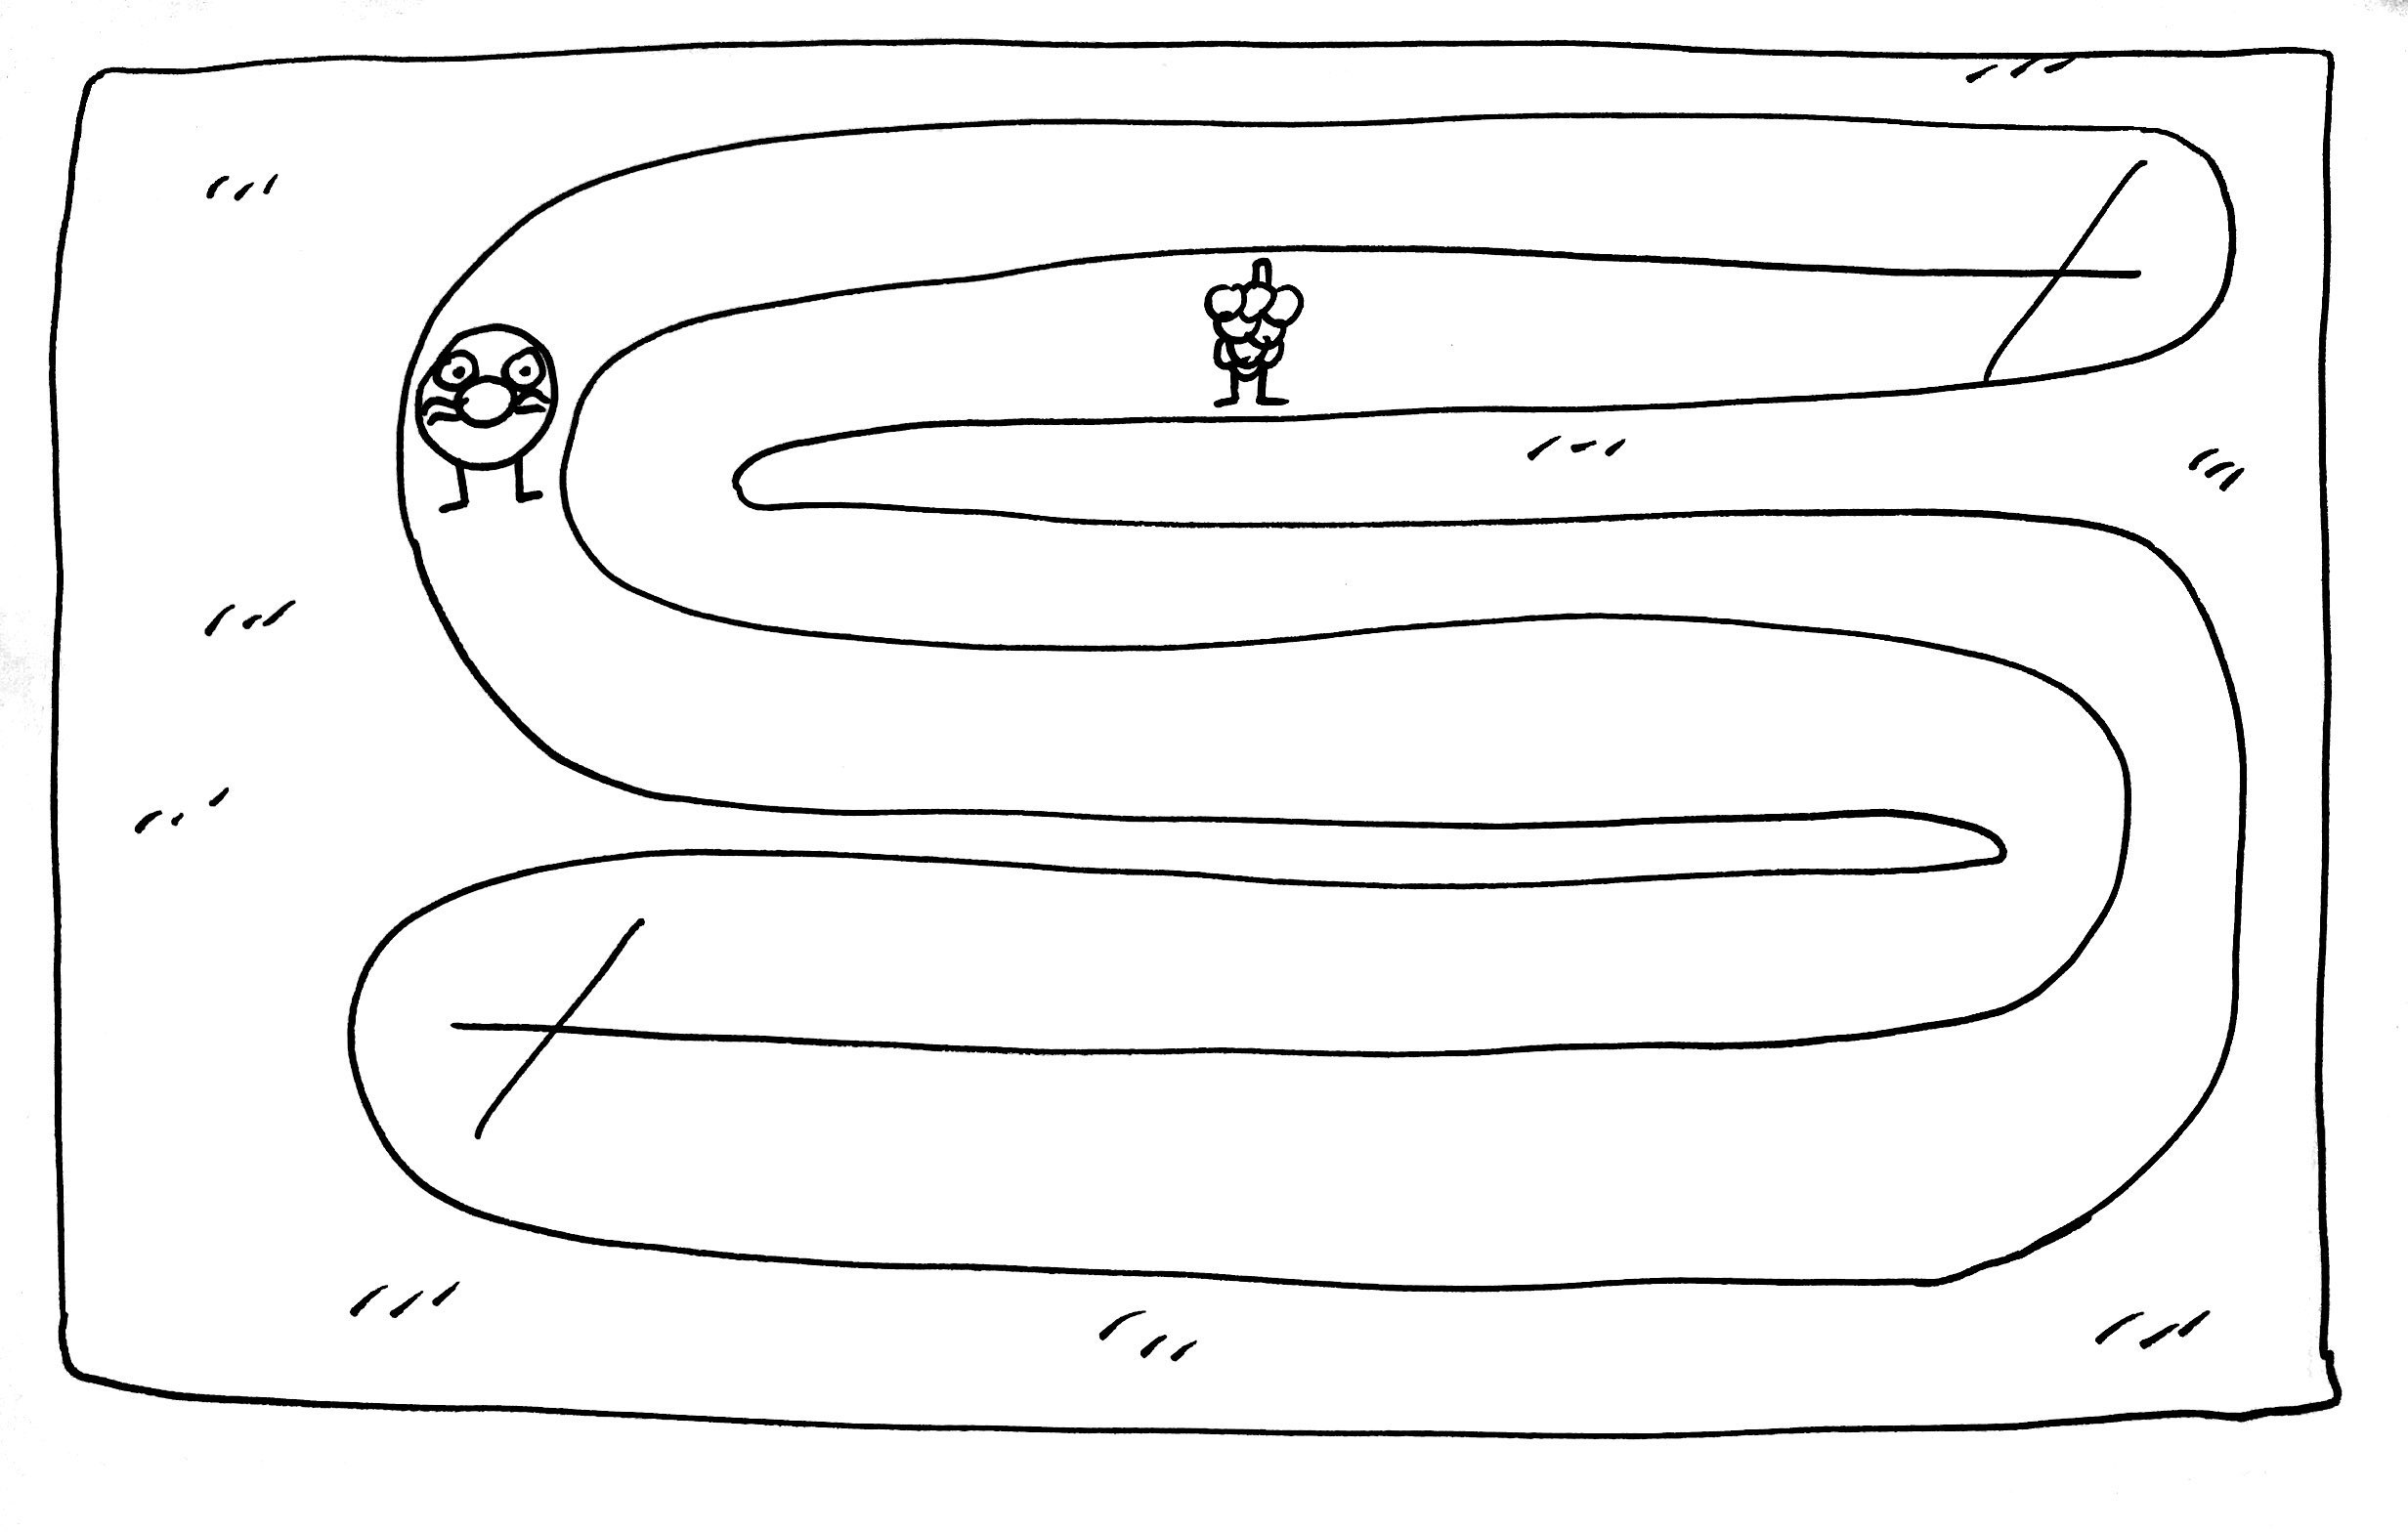
\includegraphics[scale=0.1]{Gambar/web5_gameplay2}
	\caption{Halaman pada \textit{PC} yang menunjukan berbagai permainan yang dapat dipilih.}
	\label{fig:web5_gameplay2}
\end{figure}

	\textbf{Smartphone}
	
	Halaman ini berfungsi sebagai \textit{controller} untuk para pemain. Komponen halaman ini terdiri dari dua buah gambar telapak kaki yang berfungsi sebagai tombol. Pemain dapat menekan tombol berulang kali untuk menggerakan karakter yang ada pada halaman \textit{gameplay} di \textit{PC}. Rancangan antarmuka halaman \textit{gameplay} pada \textit{smartphone} dapat dilihat pada Gambar \ref{fig:mob5_play}.
	
\begin{figure}[H]
	\centering
	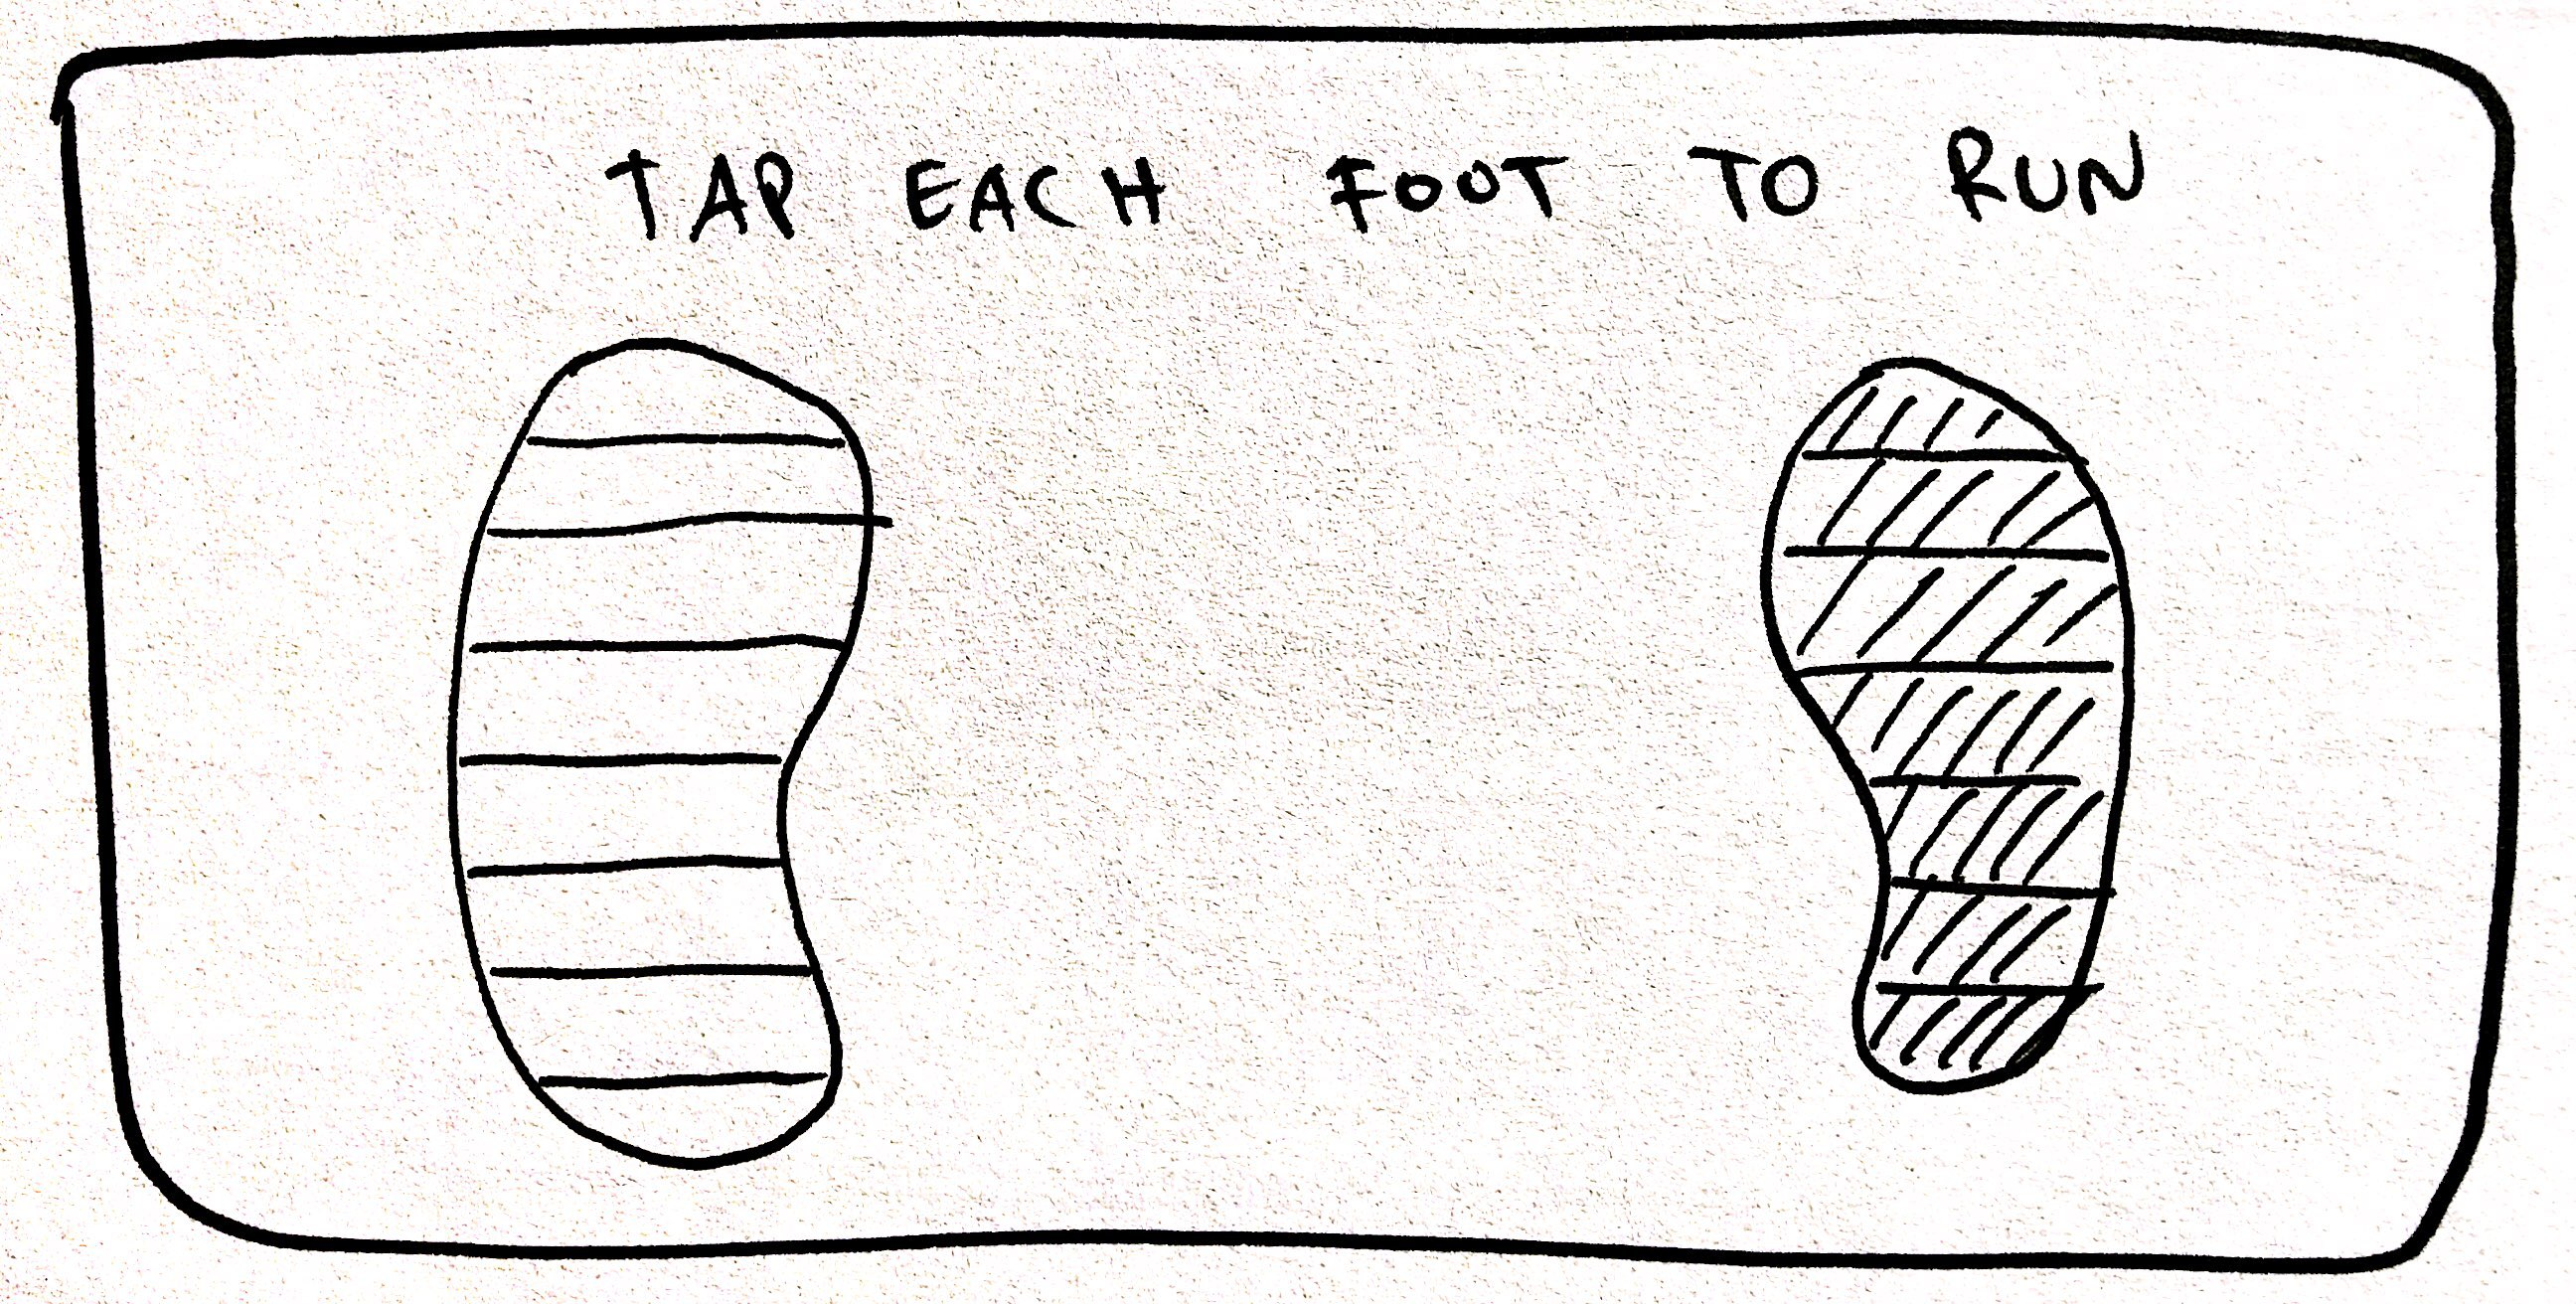
\includegraphics[scale=0.1]{Gambar/mob5_play}
	\caption{Halaman pada \textit{PC} yang menunjukan berbagai permainan yang dapat dipilih.}
	\label{fig:mob5_play}
\end{figure}

\item Antarmuka halaman \textit{gameover}

	\textbf{PC}
	
	Halaman ini menampilkan para pemenang yang telah berhasil menyelesaikan permainan. Setelah pemain selesai bermain, pemain dapat menekan tombol \textit{back} untuk kembali ke halaman utama dan mengakhiri permainan. Rancangan antarmuka halaman \textit{gameover} pada \textit{PC} dapat dilihat pada Gambar \ref{fig:web6_winning}.
	
\begin{figure}[H]
	\centering
	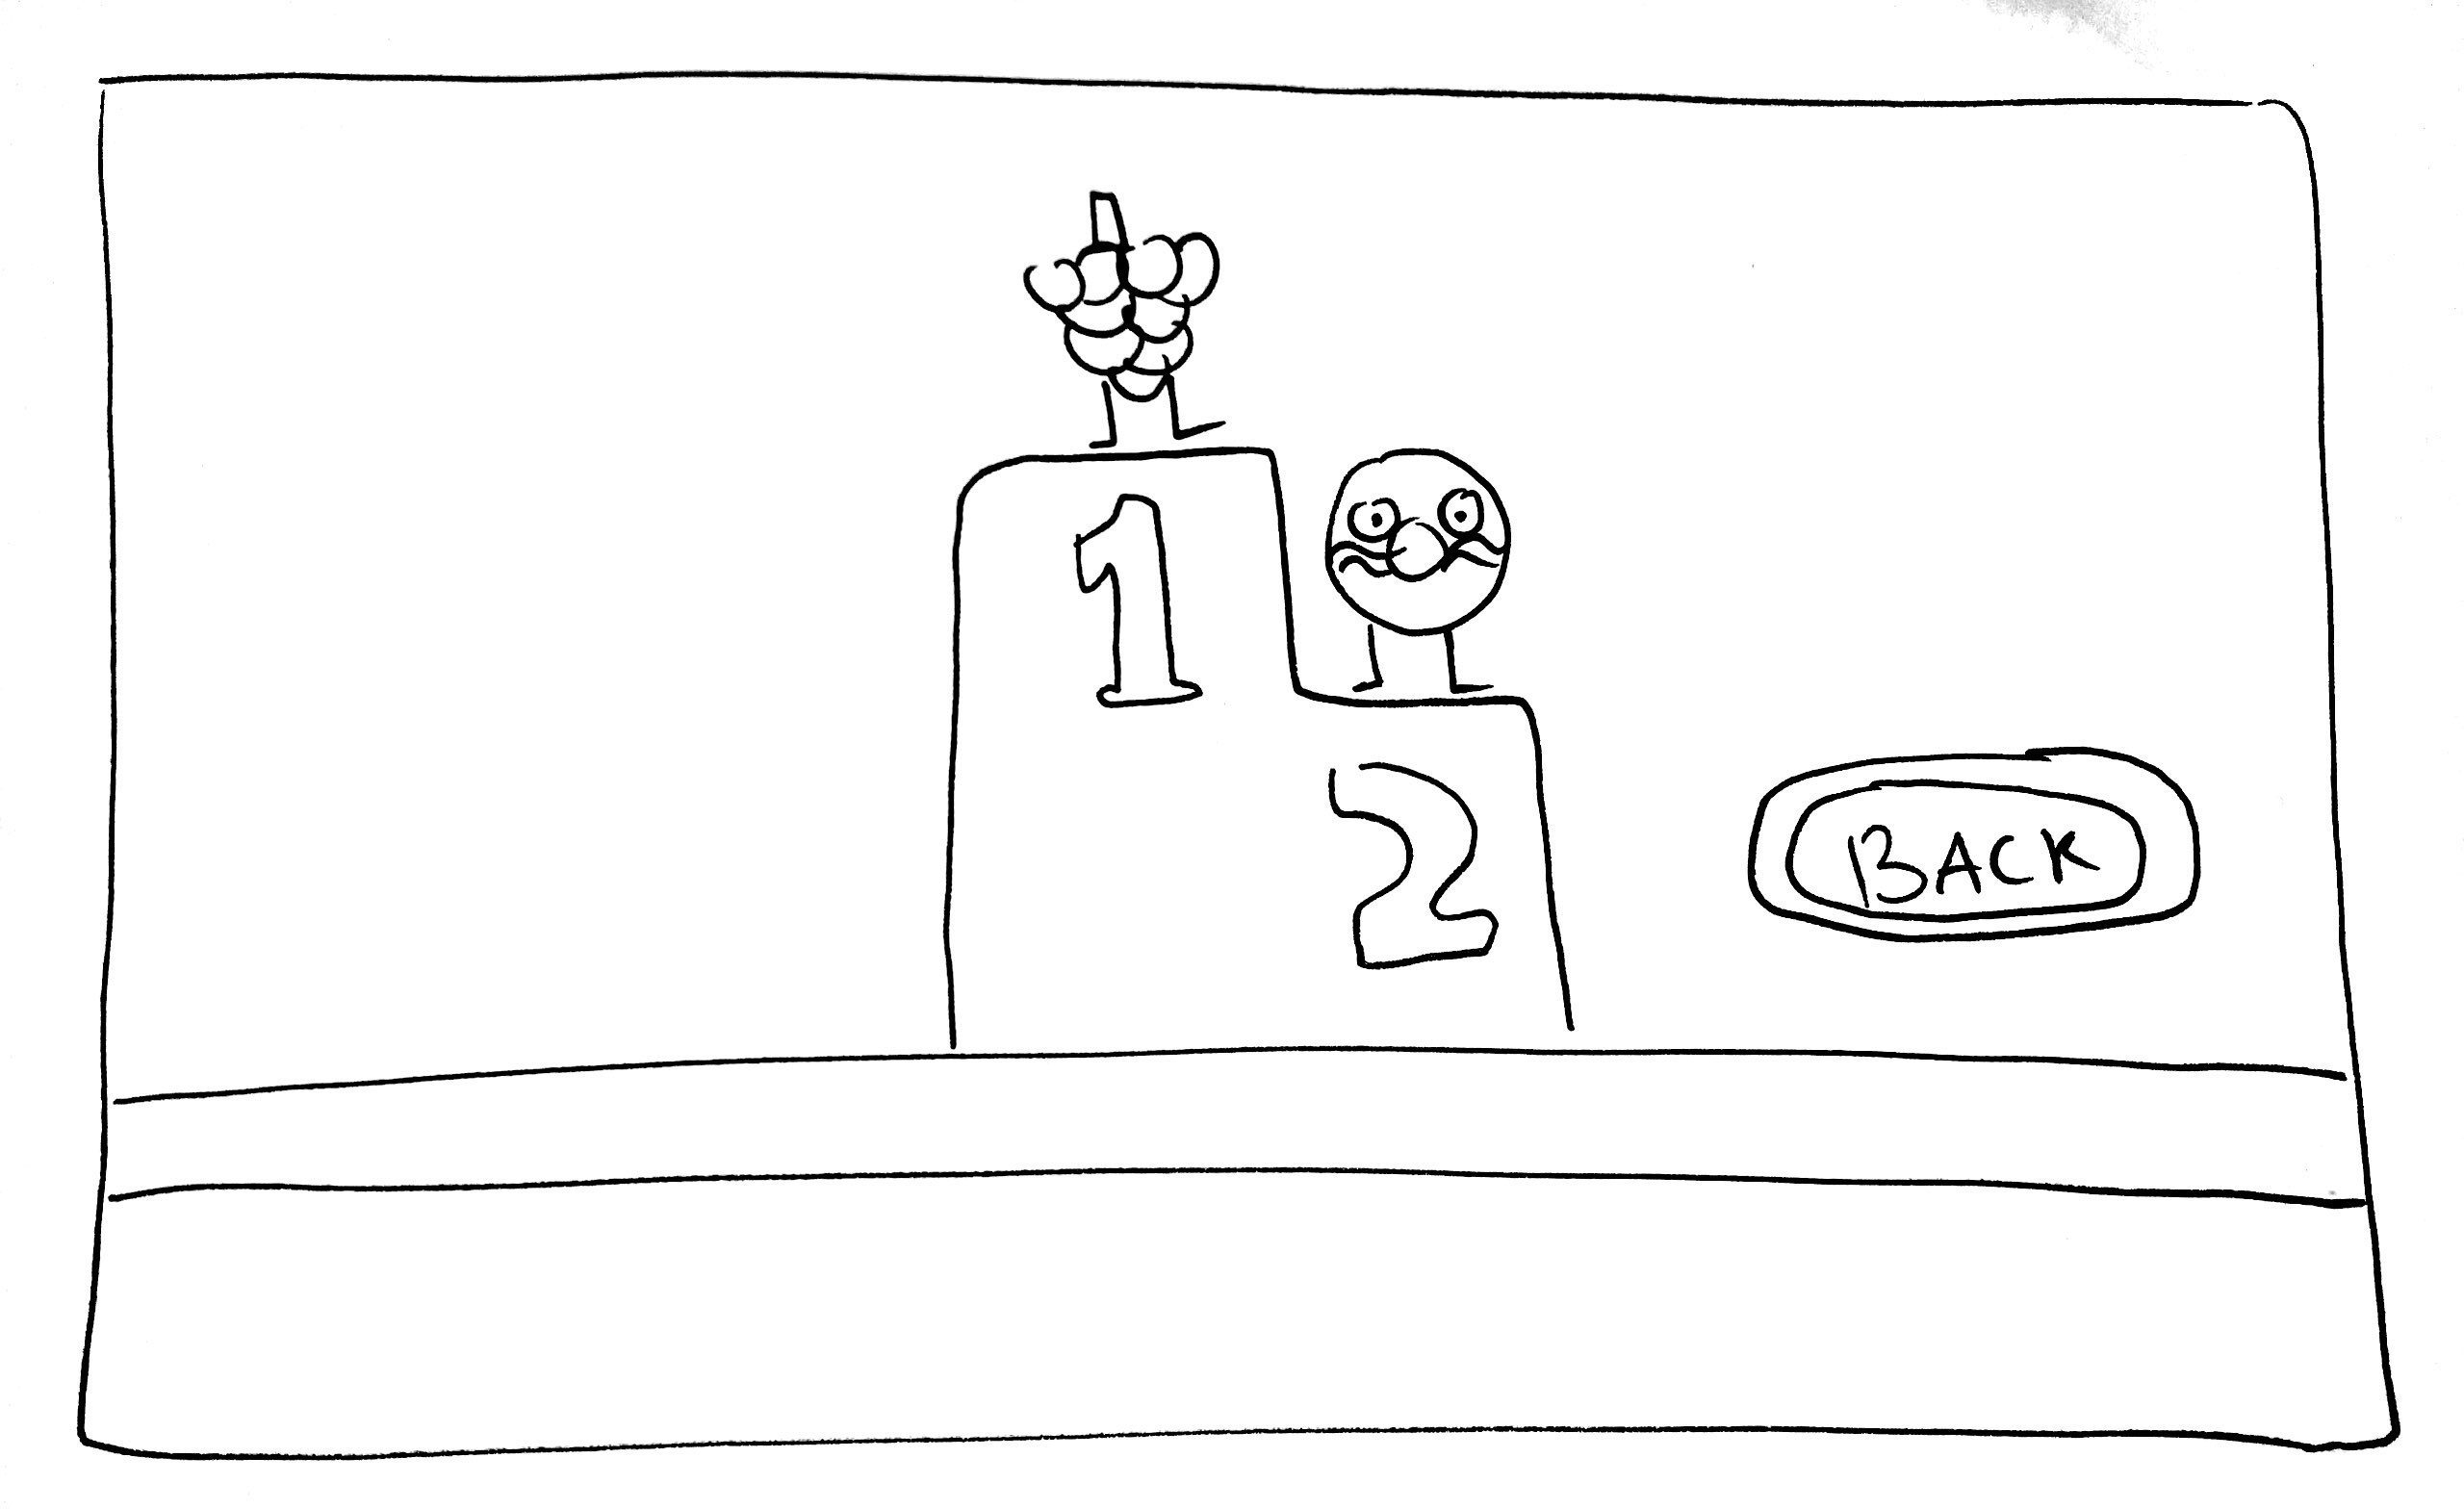
\includegraphics[scale=0.1]{Gambar/web6_winning}
	\caption{Halaman pada \textit{PC} yang menunjukan berbagai permainan yang dapat dipilih.}
	\label{fig:web6_winning}
\end{figure}

	\textbf{Smartphone}
	
	Halaman ini menampilkan teks yang menandakan bahwa permainan telah selesai. Rancangan antarmuka halaman \textit{gameover} pada \textit{smartphone} dapat dilihat pada Gambar \ref{fig:mob6_win}.
	
\begin{figure}[H]
	\centering
	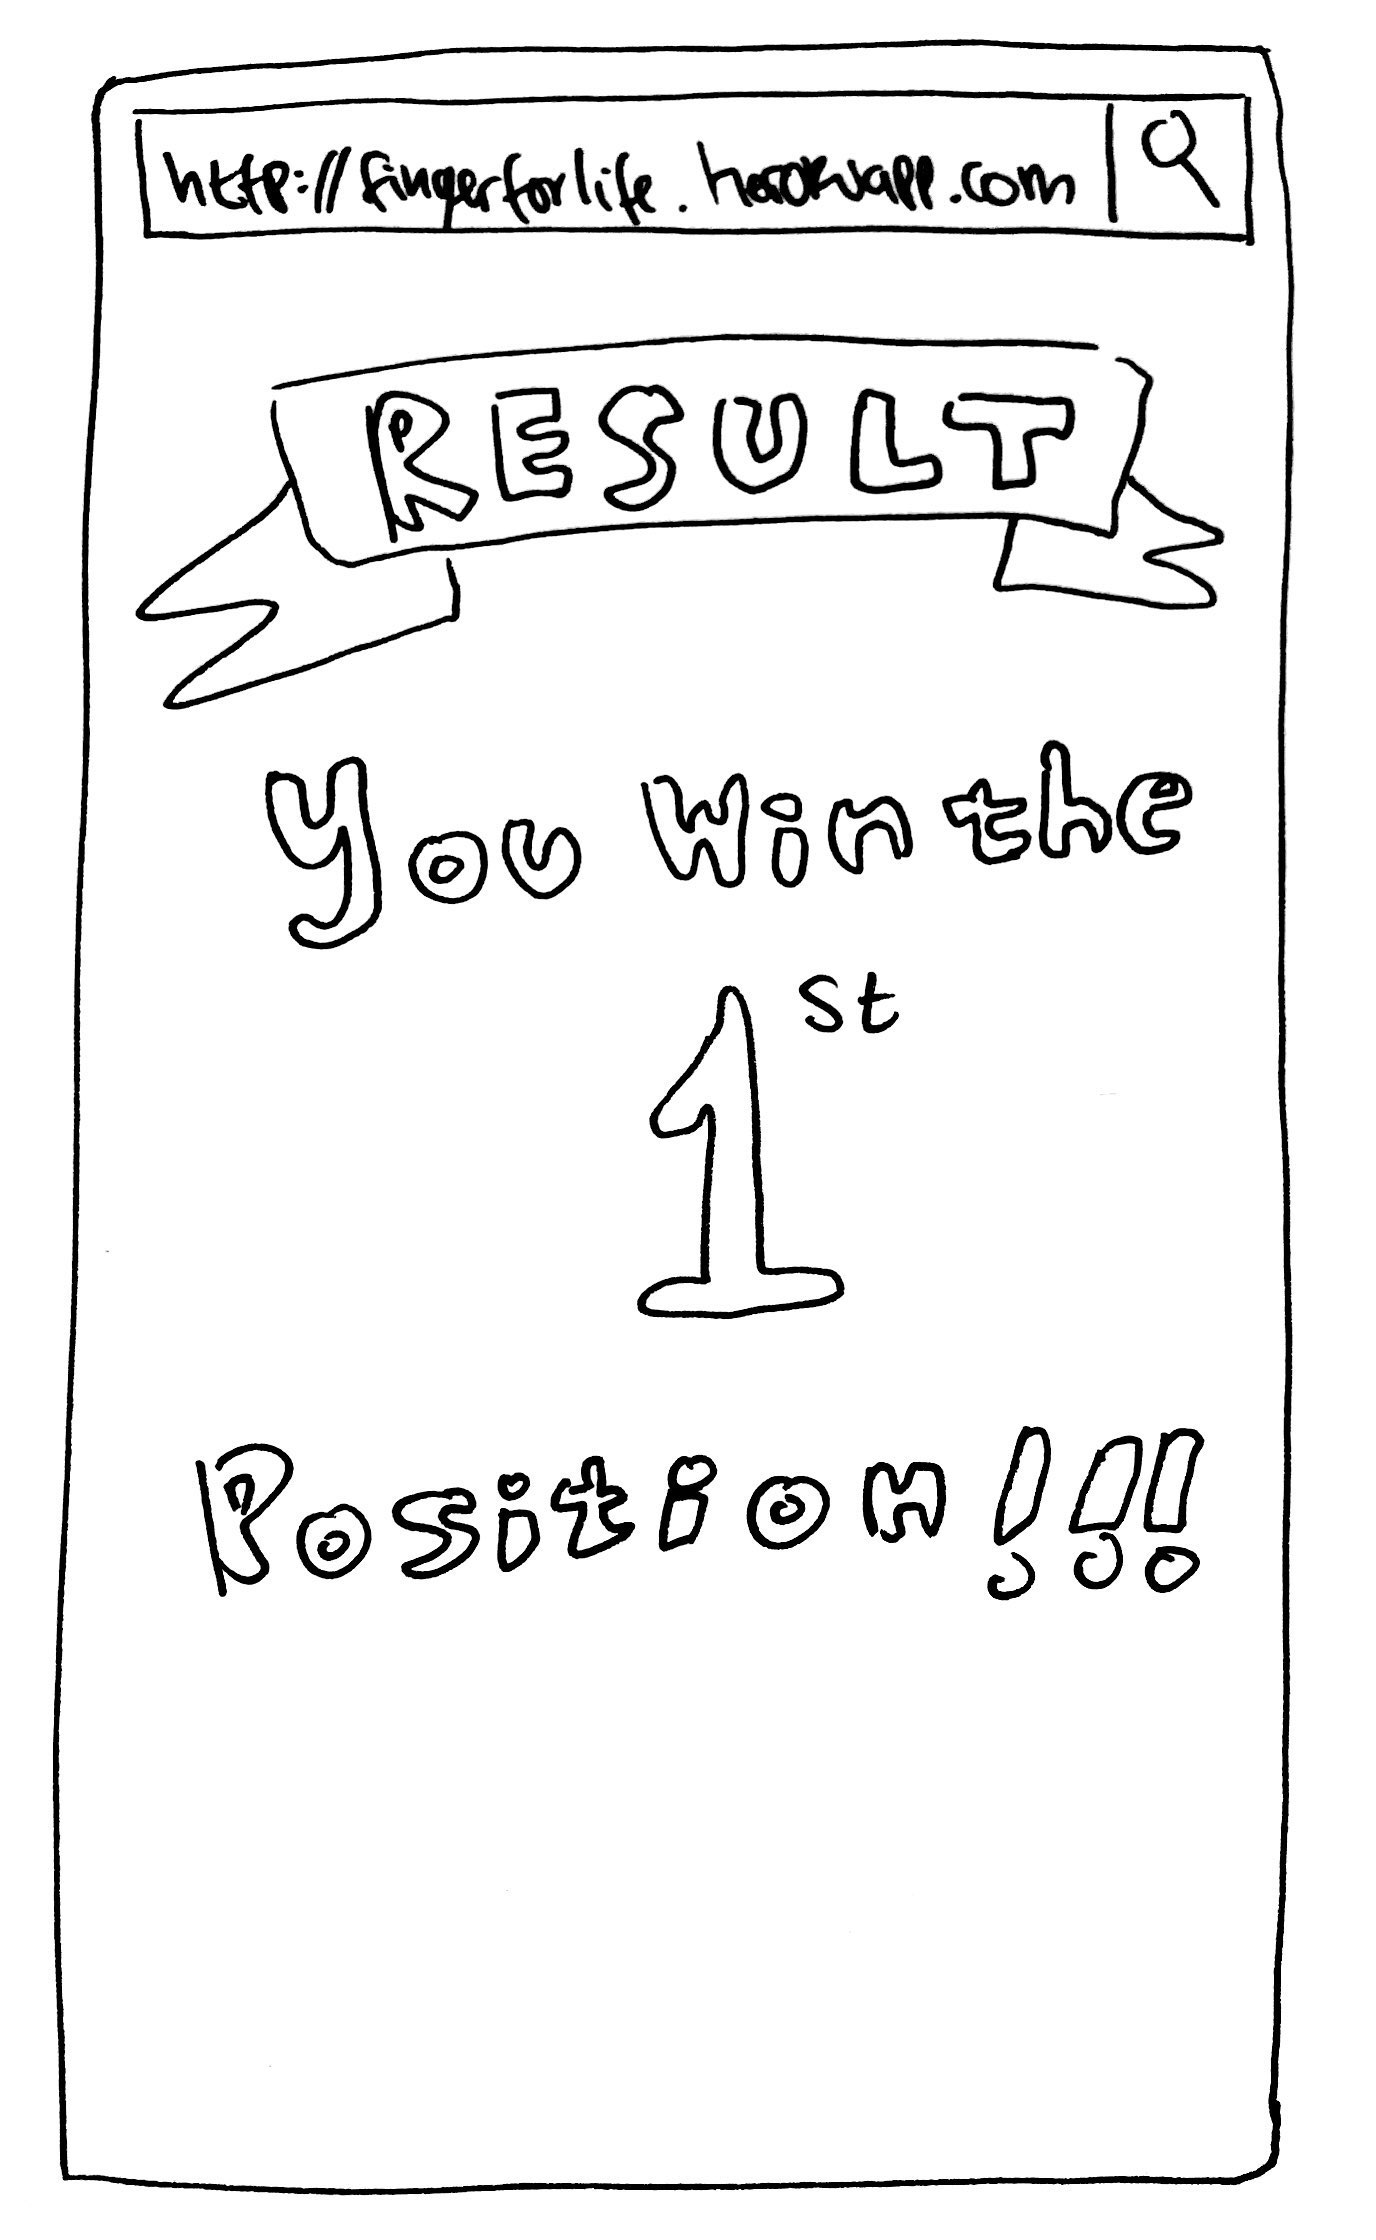
\includegraphics[scale=0.1]{Gambar/mob6_win}
	\caption{Halaman pada \textit{PC} yang menunjukan berbagai permainan yang dapat dipilih.}
	\label{fig:mob6_win}
\end{figure}
	
\end{enumerate}

\section{Perancangan Struktur Direktori}

Bagian ini akan membahas mengenai perancangan struktur direktori untuk membangun web. Struktur direktori meliputi beberapa folder dan \textit{file} yang memiliki fungsi berbeda-beda. Folder beserta \textit{file} yang digunakan akan dijelaskan sebagai berikut:

\begin{enumerate}
	\item \textbf{Folder bin} \\
	Folder ini berisi bagian-bagian yang berperan sebagai \textit{server}. Pada folder ini terdapat folder lain dan berkas yang berfungsi untuk menangani jalannya koneksi pada saat web diakses. Berikut merupakan isi dari folder ini:
	\begin{enumerate}
		\item Folder \textbf{utils} \\
		Folder ini menyimpan berkas yang membantu proses berjalannya koneksi untuk \textit{server}. Isi dari folder ini adalah sebagai berikut:
		\begin{itemize}
			\item Berkas \textbf{users.js}  \\
			Berkas ini berfungsi untuk menyimpan seluruh \textit{client} yang terkoneksi pada \textit{socket.io server}. Seluruh data pengguna yang akan memainkan permainan web akan disimpan dan diatur oleh berkas ini.
		\end{itemize}
	
		\item Berkas \textbf{www} \\
		Berkas ini berfungsi sebagai \textit{server}. Seluruh koneksi yang tersambung dan terputus akan diatur oleh berkas ini. Komunikasi antara \textit{client} pun akan diatur oleh \textit{server}.
	\end{enumerate}
	
	\item \textbf{Folder public} \\
	Folder ini menyimpan bagian-bagian yang memiliki sifat \textit{static}. Berikut akan dijelaskan isi dari folder ini:
	\begin{enumerate}
		\item \textbf{Folder images} \\
		Folder ini berisi gambar-gambar yang dibutuhkan untuk ditampilkan dibeberapa halaman yang terdapat didalam web. Berikut merupakan daftar isi dari gambar-gambar yang ada didalam folder ini: 
		\begin{itemize}
			\item \textbf{BrocoDude.png} gambar karakter brokoli dengan ukuran besar.
			\item \textbf{brocoDudeTiny.png} gambar karakter brokoli dengan ukuran kecil.
			\item \textbf{DabuDonut.png} gambar karakter donat dengan ukuran besar.
			\item \textbf{dabuDonut.png} gambar karakter donat dengan ukuran kecil.
			\item \textbf{finga.png} gambar jari yang ditampilkan dihalaman awal.
			\item \textbf{GrapeYoda.png} gambar karakter anggur dengan ukuran besar.
			\item \textbf{grapeYodaTiny.png} gambar karakter anggur dengan ukuran kecil.
			\item \textbf{stepUp.png} gambar telapak kaki kiri yang ditampilkan dihalaman pengendali.
			\item \textbf{stepUpRight.png} gambar telapak kaki kanan yang ditampilkan dihalaman pengendali.
			\item \textbf{grapeYodaTiny.png} gambar karakter anggur dengan ukuran kecil.
			\item \textbf{SummerEgg.png} gambar karakter telur mata sapi dengan ukuran besar.
			\item \textbf{summerEggTiny.png} gambar karakter telur mata sapi dengan ukuran kecil.
			\item \textbf{timer1.png} gambar angka 1 yang ditampilkan saat hitungan mundur.
			\item \textbf{timer2.png} gambar angka 2 yang ditampilkan saat hitungan mundur.
			\item \textbf{timer3.png} gambar angka 3 yang ditampilkan saat hitungan mundur.
			\item \textbf{track.png} gambar lintasan saat permainan dimulai.
			\item \textbf{winning.png} gambar panggung saat sudah ada pemenang dalam permainan.
		\end{itemize}
	
		\item \textbf{Folder javascripts} \\
		Folder ini berisi bagian-bagian yang berfungsi untuk mengatur bagaimana perilaku web pada saat diakses oleh pengguna. Terdapat berbagai berkas dengan ekstensi \textbf{.js} yang memiliki fungsi berbeda-beda. Berikut akan dijelaskan isi dari folder ini:
		
		\begin{enumerate}
			\item \textbf{Folder libs} \\
			Folder ini berisi berkas yang berfungsi untuk mengatur pengiriman data melewati \textit{form}. Berikut isi dari folder ini:
			\begin{itemize}
				\item \textbf{jquery-3.3.1.min.js} \\ Berkas ini merupakan \textbf{jquery} yang menyediakan fungsi-fungsi dalam pengiriman dan penerimaan data yang dilakukan \textit{client} dan \textit{server}. 
			\end{itemize}
		
			\item \textbf{charDesktopScript.js}, Berkas ini berfungsi untuk mengatur bagaimana perilaku halaman pemilihan karakter di \textit{desktop browser} pada saat diakses oleh \textit{client}.
			
			\item \textbf{charMobileScript.js}, Berkas ini berfungsi untuk mengatur bagaimana perilaku halaman pemilihan karakter di \textit{mobile browser} pada saat diakses oleh \textit{client}.
			
			\item \textbf{gamePlayDesktopScript.js}, Berkas ini berfungsi untuk mengatur bagaimana perilaku halaman permainan di \textit{desktop browser} pada saat diakses oleh \textit{client}.
			
			\item \textbf{gamePlayMobileScript.js}, Berkas ini berfungsi untuk mengatur bagaimana perilaku halaman permainan di \textit{mobile browser} pada saat diakses oleh \textit{client}.
			
			\item \textbf{homeScript.js}, Berkas ini berfungsi untuk mengatur bagaimana perilaku halaman utama di \textit{desktop browser} dan \textit{mobile browser} pada saat diakses oleh \textit{client}.
			
			\item \textbf{mobileScript.js}, Berkas ini berfungsi untuk mengatur bagaimana perilaku halaman proses permintaan koneksi di \textit{mobile browser} pada saat diakses oleh \textit{client}.
			
			\item \textbf{syncScript.js}, Berkas ini berfungsi untuk mengatur bagaimana perilaku halaman proses permintaan koneksi di \textit{desktop browser} pada saat diakses oleh \textit{client}.
			
			\item \textbf{winningDesktopScript.js}, Berkas ini berfungsi untuk mengatur bagaimana perilaku halaman saat permainan telah selesai di \textit{desktop browser} pada saat diakses oleh \textit{client}.
			
			\item \textbf{winningMobileScript.js}, Berkas ini berfungsi untuk mengatur bagaimana perilaku halaman saat permainan telah selesai di \textit{mobile browser} pada saat diakses oleh \textit{client}.
			
			\item 
		\end{enumerate}
		\item \textbf{Folder stylesheets} \\ 
		Folder ini berisi bagian-bagian yang berfungsi untuk menghias setiap halaman yang terdapat didalam web. Pada folder ini terdapat berbagai berkas dengan ekstensi \textbf{.css}. Berikut akan dijelaskan isi dari folder ini:
		
		\begin{enumerate}
			\item \textbf{charDesktopStyle.css}, Berkas ini berfungsi untuk menghias halaman pemilihan karakter pada \textit{desktop browser}.
			
			\item \textbf{charMobileStyle.css}, Berkas ini berfungsi untuk menghias halaman pemilihan karakter pada \textit{mobile browser}.
			
			\item \textbf{gamePlayDesktopStyle.css}, Berkas ini berfungsi untuk menghias halaman permainan pada \textit{desktop browser}.
			
			\item \textbf{gamePlayMobileStyle.css}, Berkas ini berfungsi untuk menghias halaman permainan pada \textit{mobile browser}.
			
			\item \textbf{homeStyle.css}, Berkas ini berfungsi untuk menghias halaman utama pada \textit{desktop browser} dan \textit{mobile browser}.
			
			\item \textbf{mobileStyle.css}, Berkas ini berfungsi untuk menghias halaman proses permintaan koneksi pada \textit{mobile browser}.
			
			\item \textbf{Nickname\_DEMO.otf}, Berkas ini berfungsi sebagai tipe \textit{font} yang digunakan di beberapa halaman yang terdapat pada web.
			
			\item \textbf{syncStyle.css}, Berkas ini berfungsi untuk menghias halaman proses permintaan koneksi pada \textit{desktop browser}.
			
			\item \textbf{winningDesktopStyle.css}, Berkas ini berfungsi untuk menghias halaman saat permainan telah selesai pada \textit{mobile browser}.
			
			\item \textbf{winningMobileStyle.css}, Berkas ini berfungsi untuk menghias halaman saat permainan telah selesai pada \textit{mobile browser}.
			
			
		\end{enumerate}
	\end{enumerate}
	
	\item \textbf{Folder routes} \\
	Folder ini berisi bagian-bagian yang berperan sebagai \textit{middleware}. Berikut merupakan isi dari folder ini:
	\begin{itemize}
		\item \textbf{homeRoutes.js}, berkas ini berfungsi sebagai \textit{middleware} yang menampilkan halaman utama pada saat \textit{client} mengakses alamat web. Berkas ini akan digunakan oleh berkas \textbf{app.js} yang berperan sebagai modul utama.
	\end{itemize}

	\item \textbf{Folder views} \\
	Folder ini berisi bagian-bagian yang berfungsi untuk menampilkan halaman-halaman kepada \textit{client}. Folder ini memiliki berkas dengan ekstensi \textbf{.ejs}. Sama seperti ekstensi \textbf{.html}, ekstensi tersebut akan menampilkan berbagai tampilan dengan menggunakan \textit{syntax} \textbf{.html}. Berikut merupakan isi dari folder ini:
	
	\begin{enumerate}
		\item \textbf{error.ejs}, berkas ini berfungsi untuk menampilkan halaman apabila terjadi kesalahan dalam mengakses halaman utama.
		
		\item \textbf{home.ejs}, berkas ini berfungsi untuk menampilkan halaman utama pada saat \textit{client} mengakses alamat web.
	\end{enumerate}
	
	
	\item \textbf{Berkas app.js} \\ 
	Berkas ini berfungsi sebagai modul utama, yang mengatur akses dari berbagai folder dan berkas yang ada pada struktur web ini.
\end{enumerate}